%&latex
\documentclass[11pt]{asaproc}

\usepackage{natbib}
\usepackage{graphicx}
\usepackage{amssymb}
\usepackage{setspace}
\usepackage{longtable}
\usepackage{blindtext}
\usepackage{layouts}
\usepackage[english]{babel}
\usepackage[utf8]{inputenc}
\usepackage{fancyhdr}
\usepackage{extramarks}
\usepackage{tikz}
\usepackage{algorithm}
\usepackage[noend]{algpseudocode}
\usepackage{graphicx}
\graphicspath{{images/}}
\usepackage{caption}
\usepackage{subcaption}
\usepackage{listings}
\usepackage{wrapfig}
\usepackage{adjustbox,lipsum}
\lstset{
language=R,
basicstyle=\scriptsize\ttfamily,
commentstyle=\ttfamily\color{gray},
numbers=left,
numberstyle=\ttfamily\color{gray}\footnotesize,
stepnumber=1,
numbersep=5pt,
backgroundcolor=\color{white},
showspaces=false,
showstringspaces=false,
showtabs=false,
frame=single,
tabsize=2,
captionpos=b,
breaklines=true,
breakatwhitespace=false,
title=\lstname,
escapeinside={},
keywordstyle={},
morekeywords={}
}



\usetikzlibrary{automata,positioning}


\newcommand{\alg}[1]{\textsc{\bfseries \footnotesize #1}}
\newcommand{\deriv}[1]{\frac{\mathrm{d}}{\mathrm{d}x} (#1)}
\newcommand{\pderiv}[2]{\frac{\partial}{\partial #1} (#2)}
\newcommand{\dx}{\mathrm{d}x}
\newcommand{\E}{\mathrm{E}}
\newcommand{\Var}{\mathrm{Var}}
\newcommand{\Cov}{\mathrm{Cov}}
\newcommand{\Bias}{\mathrm{Bias}}
\newcommand{\R}{\mathbb{R}}
\newcommand{\Z}{\mathbb{Z}}
\newcommand{\Q}{\mathbb{Q}}
\newcommand{\N}{\mathbb{N}}
\newcommand{\calP}{\mathcal{P}}
\newcommand{\1}{\mathbb{1}}
\newcommand{\Lagr}{\mathcal{L}}

%\usepackage{mathtime}

%%UNCOMMENT following line if you have package
\usepackage{times}

\title{Schelling Index: Measuring Decentralized Racism in the Chicago Housing Market}
\author{Daniel Silva-Incl\'{a}n}
\begin{document}


\maketitle

\begin{abstract}
This paper models decentralized segregation through a hybrid of a simple housing model and Schelling sorting in Chicago. Using Census tract data and Racial Isolation and Racial Dissimilarity indices, I estimate a racial tolerance level for Chicago in 2000 and 2010. To achieve similar levels of segregation in Chicago for both years on average, the tolerance level required is at least 50\%, which is in line with actual surveyed tolerance levels.  Consequently, there is some evidence that racial attitudes in Chicago have not changed significantly between 2000 and 2010. This is evidence that racial segregation is perpetuated by a decentralized racism, where White people pay a premium to live in a predominately White neighborhood, rather than by legal barriers, as suggested in Cutler, Glaeser, and Vigdor (1999).
\begin{keywords}
Chicago, Schelling, Segregation, Agent-Based Modeling, MCMC
\end{keywords}
\end{abstract}



\section{Introduction\label{intro}}

Economists and social scientists have a difficult time modeling and predicting the structure and growth of neighborhoods. This presents an important issue in the housing market literature, as paper after paper show that the characteristics of a neighborhood strongly affect the social and economic outcome of its residents \footnote{Racial segregation is correlated with negative outcomes for Blacks\footnote{I use the term "Black" to refer to African-Americans in this paper because most of the surveys in this paper use the term "Black" in their terminology.} in academic performance, criminal behaviors, educational attainment, employment, health outcomes, and, more simply, poverty. A short literature includes: Galster, 1987 \citep{galster87}; Case 1991 \citep{case91}; Borjas 1995 \citep{borjas95}; Orfield and Eaton, 1996 \citep{orfield97}; Shihadeh and Flynn, 1996 \citep{shihadeh96}; Cutler and Glaeser, 1997, 1999 \citep{cutler97,cutler99}; Williams and Collins, 2001 \citep{william01}; Card and Rothstein, 2006 -- 08 \citep{card06,card07,card08}.}. While researchers have studied this topic across a wide range of fields, many models of housing markets suffer from a poor balance between modeling the structural dynamics of neighborhoods, which potentially overfits the data, and omitting variables, such as underlying preferences in communities. This paper will first examine surveys to attempt to uncover the general preferences of different races. With this, this paper will examine the mismatching in survey data and empirical data through a simple housing market and additional Schelling model. Due to constraints, this paper will mostly look at Black-White racial relationships.
% * <ejz@uchicago.edu> 2016-05-11T03:39:48.550Z:
%
% > The paper will first examine surveys to attempt to uncover the general preferences of different races. With this, the paper will examine the mismatching in survey data and empirical data through a simple housing market and additional Schelling model. Due to constraints, this paper will mostly look at Black-White racial relationships.
%
% surveys are background; this does not belong in the summary. frankly I would omit this from the introduction period
%
% ^.

Several surveys in the past decades indicate that Black people are, at least, willing to live in a racially heterogeneous community. In 1982, the General Social Survey asked Blacks: ``If you could find the housing that you would want and like, would you rather live in a neighborhood that is all Black; mostly Black; half Black, half White; or mostly White?’’. On average, 67\% of Blacks chose neighborhoods that were either half Black and half White or mostly White \citep{davis92}. Similarly in the 1990s, the Multi-City Study of Urban Inequality (MCSUI) found that 50\% of Black interviewees expressed 50-50 neighborhoods as most attractive, and 99\% of them indicated a willingness to move into such neighborhoods\citep{krysan02}. Pew's 2009 reports suggest that Black people's opinion about White people has not changed much since 1990. Put another way, Black people are more likely to want to live in a heterogeneous neighborhood, and arguably even prefer white neighborhoods. However, these results could be more of an indicator that many Blacks associate White people with wealthier neighborhoods and more amenities rather than an amicability towards White people. \textit{Boondocks}, the popular comic strip and television series,  best characterized this view in their television debut with the line, ``How many times have I told you; you bet' not even dream of tellin' white folk the truth? You understand me? Shoot... makin' white people riot. You better learn how to lie like me. I'm gonna find me a white man and lie to him right now. [sic]"\footnote{One of the tritagonists, Huey is dreaming of showing White people how much their society is whitewashed the lines like "Jesus was Black", etc. He causes all the White people in the vicinity to start to brawl in disbelief of what Huey is telling them.  However, his grandfather, Robert "Granddad" Freeman wakes him up abruptly and delivers the quote above.}\citep{mcgruder05}. 

On the other side, White people have generally been less enthusiastic about integration than Black people, although White people have recently become more accepting of integration. In the previous MCSUI survey in 1990s, 60\% of White people felt comfortable with neighborhoods with one-third Blacks residences and 45\% of whites were willing to move into such neighborhoods \citep{charles03}. The General Social Survey similarly shows that White people are less eager about 50-50 type neighborhoods than Blacks, but have warmed to the idea over time \citep{schuman97}. Overall, White people are increasingly agreeing with the principle that Blacks should be able to live wherever they can afford, although a substantial minority still have their reservations\citep{schuman97,bobo01}. This echoes similarly to the logic of ``Not in my backyard'' where White people say they want Blacks to succeed --- just not near them. It is worth noting that evidence from Detroit seems to indicate that Whites are more willing to remain in their neighborhoods as Blacks enter than they used to be \citep{farley94}. However, when studies found a clear White preference for segregation, the housing market opportunities of Black and Hispanic households were substantially reduced \citep{farley94,bobo96,charles00}. It is also possible, however, that Whites are understating their taste for discrimination in these surveys. Similarly, the recent popularization of politically correct language may mask the true opinions and tastes for discrimination with politeness and platitudes.

Regardless, there is a strong discrepancy between survey responses on race preferences and the actual composition of neighborhoods. The actual composition of neighborhoods is driven by more than just traditional drivers of housing choice, like income. Rosenbaum finds that, after controlling for demographic and economic differences, Blacks reside in lower quality housing and neighborhoods than Whites\footnote{For more information on race preferences see Farley et al. (1978, 1994)\citep{farley78,farley94,farley94b}} \citep{rosenbaum99}. 1990 Census data suggests that the segregation between Blacks and White people in many US cities cannot solely be explained by racial income differences\citep{massey93}. The 1989 Housing Discrimination Study (HDS) found that in both rental and owner-occupied housing markets, Blacks faced significant levels of discrimination\citep{yinger95}. The HDS also conducted their study again in 2000 and found that disparate treatment discrimination in rental and owner-occupied housing markets has been reduced by an order of magnitude over the last decade. However, they find key exceptions to their result in discrimination against Hispanics in access to rental housing, racial steering of Blacks, and less assistance to Hispanics in obtaining mortgages. Other researchers have also found evidence of similar discriminatory behaviors within US housing markets and only modest steps towards integration in the 2000 census\citep{glaeser00,ross05a,turner05}. What is clear is that there is some additional factor driving the market. It is possible that there are other preferences correlated with race, or that there is some hidden financial reason that explains the difference. 

The housing market literature has mixed results on what specific mechanisms cause segregation in housing markets. Cutler, Glaeser and Vigdor (1999) find that segregation has declined since 1970, as Blacks moved into previously all-White areas of cities and suburbs \citep{cutler99}. To some extent, the decline of segregation could be attributed to the Fair Housing Act in 1968, among other legislation, which allowed Blacks to more freely choose their homes. While overall segregation has been reduced, there are also more all-black neighborhoods than before, which drives an increase of the variance of segregation levels of US cities while lowering the mean. Regardless, Cutler et. al. (1999)  find evidence that in 1990 and beyond, the legal barriers which enforced and perpetuated segregation were mostly replaced by a decentralized racism, where whites pay more than blacks to live in the predominantly white neighborhoods \citep{cutler99}. These findings, as well as Bill Rankin's Maps of Chicago, are the primary motivation for this paper.

\section{Literature}

The model in this paper is influenced by several disciplines, including Urban Economics, Geography, Regional Science, Social Psychology, and Computational Sociology. While these disciplines are interested in modeling neighborhoods, they seem disconnected, evidenced by several paths and languages for identical or similar insights. For example, whereas regional science describes ``social energy''\citep{isard72}, economics has ``shadow prices,'' -- both of which provide the same argumentative work. Despite the unfortunate consequences of a failure to communicate between disciplines, there are still examples of insights unique to a single field. Hence, a multipronged approach may allow us to better reproduce the salient features of the housing market.

Most economists (and several researchers from other fields) study segregation through statistical regressions. The statistical regressions approach involves inferring relationships of raw data, indexes, and factors though statistical modeling based in some sort of regression analysis. However, to better capture the underlying mechanisms in housing markets, researchers need to model the problem more dynamically. Statistical modeling is very good at answering questions of correlation and significance. However, without some underlying theory in the model, statistical modeling is easily prone to spurious relationships and simple nonsense.  One alternative approach is structural econometric modeling, in which regressions are built around a theoretical model. A large number of mostly economic papers follow the Price Theory framework for their structural models, which constructs markets and economies of maximizing actors often with rational expectations.\footnote{Specifically, they model housing market through the work of Alonso 1964\citep{alonso64}, Mills (1967, 1972b)\citep{mills67,mills72a,mills72b}, and Muth 1969\citep{muth69}, which is built around optimizing the commuting cost differences within an urban area with the price of living there. The focus of of modeling this way, as Glen Weyl describes it, is:``an analysis that reduces rich (e.g. high-dimensional heterogeneity, many individuals) and often incompletely specified models into `prices’ sufficient to characterize approximate solutions to simple (e.g. one-dimensional policy) allocative problems." \citep{weyl15}. These price-theoretic papers model the dynamical nature of the economic system generally at the cost of complexity.} Price-theoretical models tend towards a Beckerian analysis in which the agents have a taste for discrimination and pay for it via opportunity cost. More recently, a small number of papers now follow the agent-based model (ABM) approach which may better capture the underlying dynamic process in housing markets. The ABM approach is built on simulations rather than regressions, but as a result it also requires a predictive economic model, thus also avoiding the pitfalls of simple regression analysis.  

Starting with Conway's ``Game of Life" in 1970 and Schelling's ``Dynamical models of segregation" in 1971, ABM models focus on using a foundation of simple rules to simulate complex behavior\citep{conway70,schelling71}. This is in contrast to the more traditional economic models, where the key modeling unit is a representative agent. ABM models allows the researcher to better focus on the heterogeneity within the system that may not be easily deduced by simply aggregating the properties of the agents. Additionally, in ABM models, the system in question is reduced to simple rules of interaction between agents and objects rather than mathematical equations that may be intractable or largely composed of florid distractions. In Conway's ``Game of Life'', there is simply a grid, two states for each box, and four simple rules. However, from even these simple simulations, complex behaviors can emerge. Several papers on evolutionary development, ecosystems, and swarming followed based on merely small changes to Conway's basic model. Schelling's segregation model, a similarly simple but powerful model, also provides the unfortunate insight that preventing segregation is a more difficult problem than originally thought. Even with simple rules for moving and only light prejudice, ``cities'' can become highly segregated\citep{schelling71}. \footnote{It is worth noting that although the Schelling model does endow agents with preferences, it does not impose an opportunity cost on acting on those preferences, which may explain why Schelling's model predicts higher levels of segregation than Becker's model. Zhang address some of these issues\citep{zhang11}}

\section{The Rise and Decline of the American Ghetto}
Cutler \textit{et. al.} (1999) examine segregation in American cities from 1890 to 1990 using regression analysis and two novel segregation indices. The first, Bell's (1954) racial isolation index, measures the degree of isolation of a certain race among neighborhoods\citep{bell54}. The second, the Racial Dissimilarity index, measures the evenness in which two mutually exclusive groups are distributed\citep{duncan55}. Although these measures are not without critics, they are widely used in Urban Economics and Sociology.

\begin{equation}
\label{eq:rii}
\mbox{Racial Isolation Index} = \frac{\sum_{i=1}^N\big(\frac{black_i}{black_{total}}\cdot\frac{black_i}{persons_i}\big)-\big(\frac{black_{total}}{persons_{total}}\big)}{\min\big(\frac{black_{total}}{persons_l},1\big)-\big(\frac{black_{total}}{persons_{total}}\big)} .
\end{equation}

Similarly,

\begin{equation}
\label{eq:rdi}
\mbox{Racial Dissimilarity Index} = \frac{1}{2}\sum_{i=1}^N\bigg|\frac{black_i}{black_{total}}-\frac{nonblack_i }{nonblack_{total}} \bigg| .
\end{equation}

{\setlength{\parindent}{0cm}Note that both indices are between 0 and 1. As Cutler et, al. point out, there are several other ways to measure segregation levels, but they tend to require additional information which is not readily available such as clustering and centrality.
}

Cutler \textit{et. al.} (1999) explore three theories on why \textit{ghettos} develop, sustain, and even perpetuate themselves. For brevity, each segregation theory is defined and evidence for each theory is in the respective footnote. The first theory is known as the \textit{port of entry} theory, where minorities prefer to live among members of their own race, especially when they are new migrants. Potential forces for this include a preference for cultural or religious homogeneity, and language barriers, among others \footnote{Evidence for this theory includes, according to the General Social Survey, after 1970, Black migrants from the South into the North were 10\% more likely to belong to an all-Black church than native Northern Blacks and 24\% more likely to prefer to live in a segregated neighborhood. Sociology and Anthropology use the concept of `the Other' to explain this phenomena \citep{mead62}.}. In other words, ghettos help immigrants assimilate into the new environment. The second is the \textit{structural racism} theory, where mostly Whites use legal, quasi-legal, and/or violent illegal barriers to keep minorities out of white neighborhoods\footnote{Jim Crow Laws in the South (1890 - 1965), Stop-and-Frisk in NYC (1990 - 2014, known as Stop-Question-Frisk in 1990s), vigilante lynching throughout the US (1882 - 1959) are examples of each group respectively\citep{black03}. More examples of legal and quasi-legal legislation affecting race-relations include the millions of Native Americans systematically forced into reservations under Manifest Destiny ideology (19th Century), thousands of Mexicans absorbed through the Mexican-American War in 1847, and the Chinese Exclusion act of 1882 - 1943 which disallowed Chinese immigration and naturalization. Examples more specific to housing include racial zoning or restrictive covenants prohibiting sales to African-Americans, firebombing, and later red-lining (restricting access to credit markets)\citep{spear67}. In short, race integration in the US has been a messy, violent, and incomplete process \citep{black03}.}. The third is the \textit{decentralized racism} theory, where whites segregate themselves by paying more to live with members of their own race\footnote{For purposes of Cutler \textit{et. al.} (1999) and this paper, racism does not connote a belief in the inherent superiority or inferiority of a racial group. Rather, it refers to the Beckerian notion of discrimination where an individual has a taste for a particular type of neighborhood racial composition.}. Cutler \textit{et. al.} determined the type of segregation that was underlying each housing market within cities by comparing the attitude towards immigration and the price discrimination in the housing market. Table \ref{tab:cutler6} shows the predictions for the alternative theories of segregation. Cutler \textit{et. al.}  finds that throughout 1890 -- 1990, Blacks tended to pay more for similar houses as Whites, while Whites had stronger preferences for segregation than Blacks. However, by 1990, Whites tended to pay more for segregation and still retained their racial preferences. Hence, Cutler \textit{et. al.} conclude that decentralized racism has become key in American cities since the 1990s. Other researchers have found similar evidence for structural racism in the housing market \footnote{Weaver, 1948\citep{weaver48}; Duncan and Duncan, 1957\citep{duncan57}; King and Mieszkowski, 1973\citep{king73}; and Yinger, 1978\citep{yinger78}; and Reifel, 1994\citep{reifel94}}.

\begin{table}[h!]
\begin{tabular}{|p{3cm}||p{3cm}|p{3cm}|p{3cm}|p{3cm}}
\hline
\multicolumn{4}{|c|}{Predictions of Alternative Theories of Segregation}\\ \hline \hline
 Relationship between segregation and: & Port of Entry & Structural Racism & Decentralized Racism\\
 \hline
  House Prices & Blacks pay more (esp. migrants) & Blacks pay more & Whites pay more\\
  & & & \\
   Attitude towards immigration & Blacks prefer segregation (esp. migrants) & Whites prefer segregation & Whites prefer segregation\\
 \hline \hline
\end{tabular}
\caption[Alternative Theories of Segregation]{Predictions of Alternative Theories of Segregation (source: Cutler \textit{et. al.} 1999, Table 6)}
\label{tab:cutler6}
\end{table} 

All three theories are based in Becker's taste-based and statistical theories of discrimination \citep{becker10}. In taste-based discrimination, individuals bear a non-pecuniary cost from associating with a particular group, often their own. In contrast, by statistical discrimination, there are perceived, and accurate, statistical differences between groups, which act to separate racial groups in their interactions in the presence of imperfect information about individuals. Figure \ref{fig:income} shows that most Whites (not Hispanics) can to price out most minority (except Asian-American) residents if they so choose. The ratio between Black real median household income and white real median household income has not changed in the last 50 years. Similarly, with restrictions on the credit market Blacks have faced with red lining, it is not surprising that desegregation has been slow to reach housing markets.

\begin{figure}[h!]
\centering
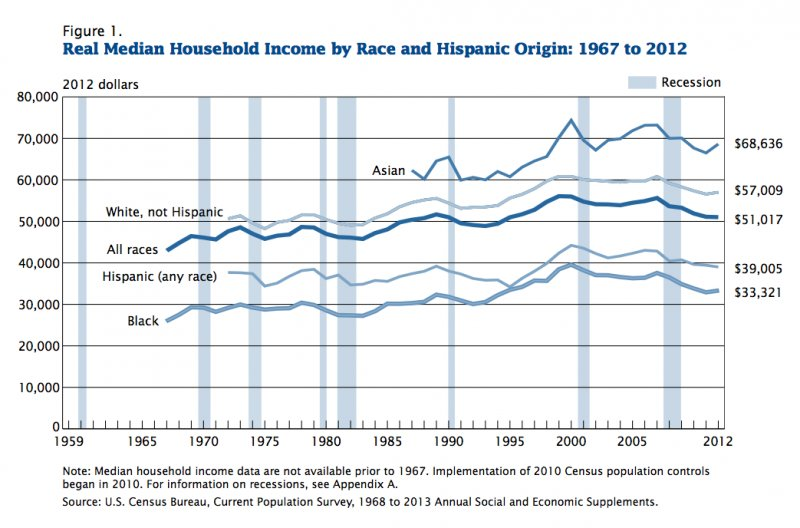
\includegraphics[width=14cm]{figures/Household_Income.png}
\caption[Real Median Household Income]{Real Median Household Income by Race and Hispanic Origin: 1967 -- 2012}
\label{fig:income}
\end{figure}

Social psychologists have developed their own theories of agents' racial preferences which further explains the mechanism of discrimination. Based on the empirical research of Henri Tajfel and John Turner, their theories shed light on segregation at the macro level\citep{tajfel79}. They define in-groups, or a group that one identifies with and is a member of, and out-groups, or groups that one is not a member of, to model prejudice and discrimination. Tajfel's Social Identity Theory claims that social categorizations systematize the social world and provide the agent with a system of self-reference. As such, the agent defines their identity and self-image from the social categories that he perceives himself belonging to. These categories may arise due to shared interests, shared racial categories, and enforcement by societal norms and authority, among other factors. Empirically, agents exhibit in-group favoritism, or a preference and affinity for one's in-group over the out-group even when the groups are arbitrarily constructed. This is potentially best shown in Jane Elliot's ``Blue eyes–Brown eyes" exercise\footnote{The Blue eyes–Brown eyes exercise aims to simulate discrimination. Specifically, a group of people was divided up based on their eye color. One group was deemed the privileged group and received benefits while the other group was treated poorly. Interaction between the two groups were discouraged and the non-privileged class had similar restrictions as African-Americans had before civil rights, such as being forced to sit in the back or drink from a different water fountain than Whites. It's worth noting that Elliot's exercise is not always successful in inducing discriminatory sentiment and has potential ethical issues (her sample was elementary school students). However, Elliot's work provides some evidence of the artificial nature of discriminatory sentiment.}. Moreover, agents exhibit out-group derogation, a phenomenon in which an out-group is perceived as being threatening to the members of a group. These empirically observed behaviors suggest the importance of incorporating class and racial preferences into the study of segregation. In-group members will strive to live with each other and move away from out-groups with different races, backgrounds, and interests. Regardless of the approach, we have a theory of why discrimination may exist at the individual level, manifested in preferences, and social level, manifested in segregation.

\subsection{Radical Cartography}

\begin{figure}[!h]
\centering
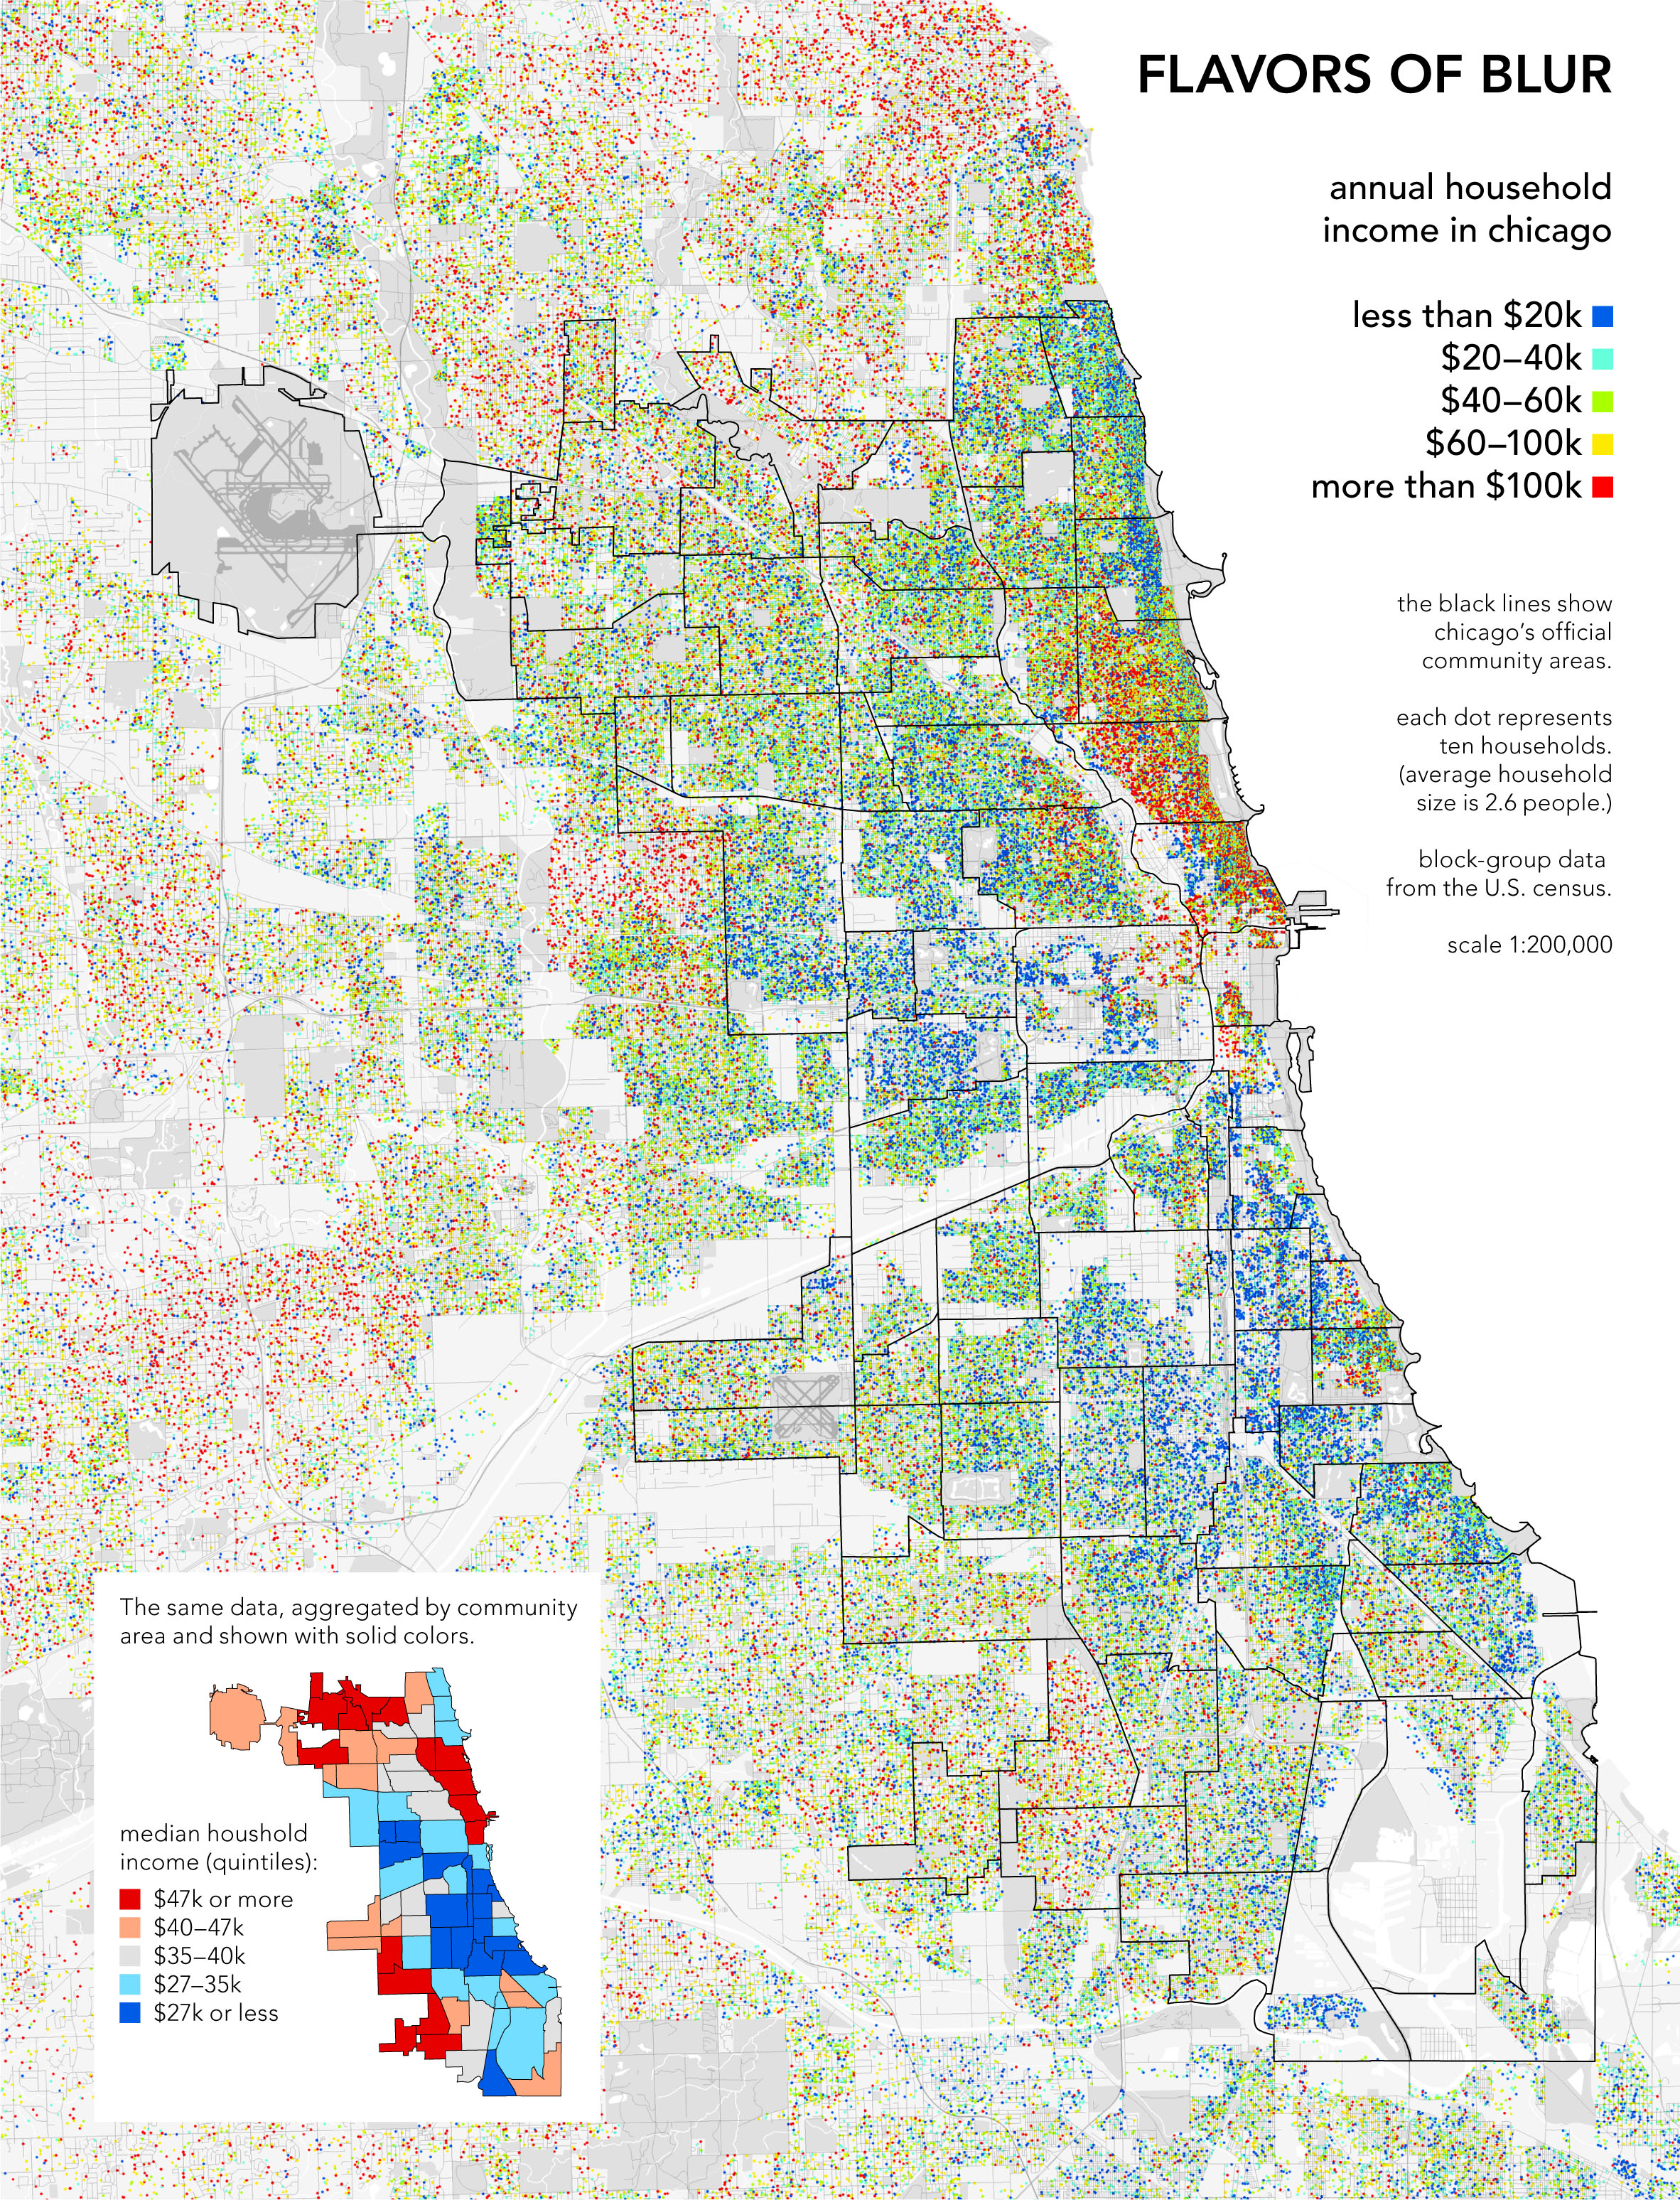
\includegraphics[scale=.32]{figures/chicagodots_income_big.jpg}
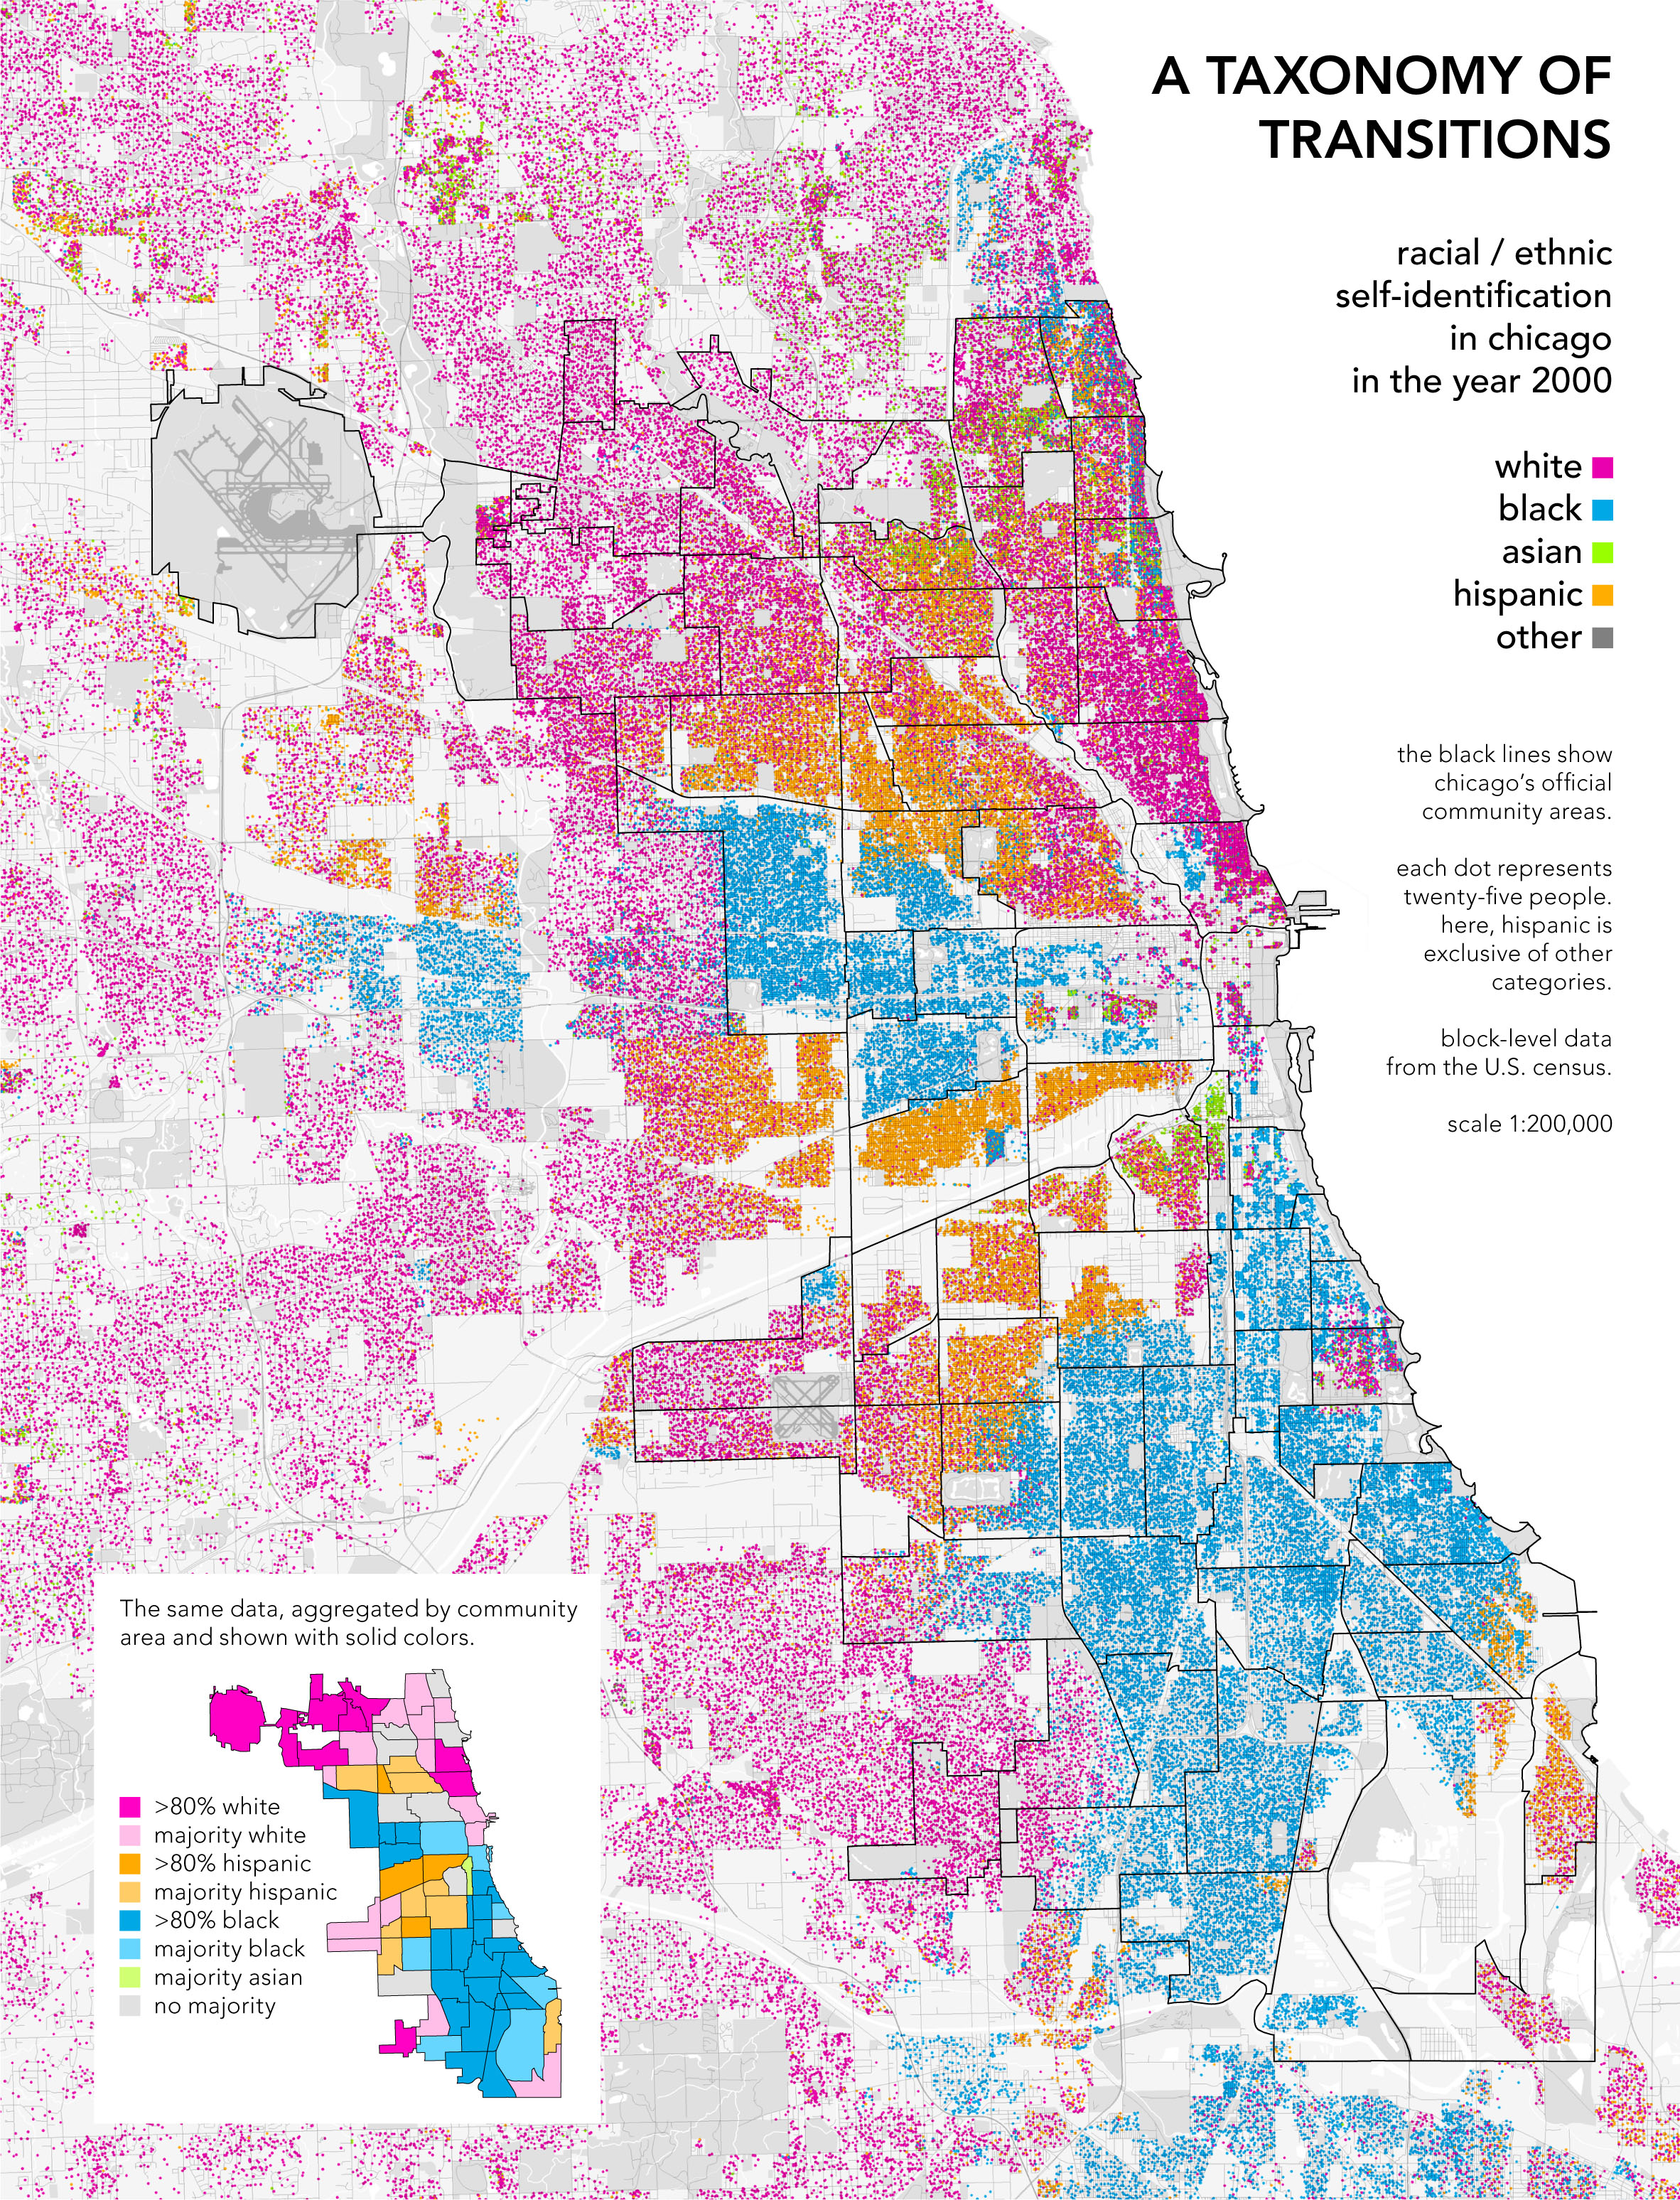
\includegraphics[scale=.32]{figures/chicagodots_race_big.jpg}
\caption[Bill Rankin's Income and Race Maps of Chicago]{Bill Rankin's Income and Race distribution maps in Chicago (Source: Radical Cartography)}
\label{fig:rankin}
\end{figure}

Schelling's individual agent grids are best thought of as Pointillist maps, which have recently become popular with social scientists due to the work of cartographers like Bill Rankin. Unlike many other cartographers, Rankin focuses on destabilizing the traditional political undertones present in line-boundary maps. More precisely, he rejects the old mantra in cartography of strongly politically defined boundaries in favor of more measurable criteria. As Rankin writes: ``Boundaries lead a dual life: they are described as `imaginary lines,' often with no physical presence except on a map, but they also have very real effects on people, nature, and territory." \citep{rankin10}. Simply put, choosing which map to use influences not only our interpretation of the area but also influences the real development of the area itself. This is not a new idea, but Rankin and later Eric Fischer\footnote{Eric Fischer is a data artist and software developer at Mapbox. He has a photograph blog on Flickr with over 7.3k followers where he presents his racial Pointillist maps, among other things.} have become prominent in their respective fields with this work. 

Rankin creates a Pointillist style map where he represents agents as dots. This is in contrast to presenting the spacial demographics of a city by the ridge census tracts, which are a step removed from the individuals and may have political undertones in their form. The Pointillist style map allows the presentation of the agents to be more fluid and organic. The maps are technically more accurate as well because they emphasize each agent's location and identity rather than a superimposed framework. Comparing Rankin's maps with the traditional census map in figure \ref{fig:rankin}, the Pointiliist style map shows the smoothness and transition in greater detail. For purposes of this paper, this cartographic ideology allows us to use Tiebout's intuition of people ``voting with their feet" to attempt to capture the underlying economic phenomena rather than capturing the structure of the census blocs \citep{tiebout56}. Perhaps because Rankin is a cartographer and not a statistician, Rankin only presents qualitatively the difference between Pointillist style maps and the traditional variants\citep{rankin10}. He does not present an explicit error rate in the traditional census map versus a Pointillist map. This sort of analysis could potentially be useful to check whether this additional level of resolution would be beneficial in other scenarios. However in this case, there are clear gains and a simple integration to be had by integrating Rankin's radical cartography with a rigorous Schelling model.

\subsection{Tipping and Residential Segregation: A Unified Schelling Model}

Zhang (2011) \citep{zhang11} updates the Schelling model by both adding mathematical rigor and expanding upon some complications. Specifically, he models Schelling in a context of no racial discrimination wherein both Black and White agents prefer to live in 50-50 neighborhoods, and wherein socioeconomic disparities between white and black agents are completely eliminated. The mathematical rigor of the simulation allows for stronger proofs of the effects than Schelling's simulated examples. Zhang also clarifies some potentially nebulous definitions. Furthermore, Zhang facilitates extensions of the Schelling model, as now the richness of evolutionary game theory can be more easily implemented. As Zhang remarks, Young (1998) was the first to argue that the techniques developed in evolutionary game theory are useful for analyzing Schelling’s segregation and spacial models\citep{young98}. Foster and Young (1990) develop the concept of stochastic stability which is a rigorous analysis of long-run solutions in evolutionary game theory\citep{foster90}. Young (1998, 2001) presents a simple variation of the one-dimensional Schelling model on a ring\citep{young98,young01}. He shows that segregation tends to appear in the long run even though a segregated neighborhood is not preferred by any agent.

Zhang rigorously shows that stark segregation is a steady state in the situations he explores. The agents are in a Tragedy of the Commons game where no one or no set of agents is willing or able to take the necessary steps to ensure to maximize social or individual utility. Hence, the Nash equilibrium is not Pareto Optimal. It seems that unless there are very strong preferences in multiple agents for integration or a dictator-like social planner, segregation will persist in this model. Similarly, Zhang shows that the initial conditions are relatively invariant as both random start and `ghetto' starts lead to similar levels of segregation\footnote{In a random start, all the races are randomly mixed on the board. In a ghetto start, the Black population is concentrated at the center of the city.}. An important extension for Zhang is the inclusion of a housing market and heterogeneous agents in terms of wealth. This paper continues on that path.

\section{Model and Simulation}

Consider a $Y \times X$ bounded lattice graph where $X,Y \in N$. For simplicity, let $Z = YX$. In each vertex, there is a single residence for a single agent. We allow for vacant houses, hence, there are $Z$ houses and $N$ agents where $N \leq Z$. Agents are defined by a their race, $r\in\{$White, Black, Hispanic$\}$ and income $w$. This paper simplifies the wealth distribution with the function $w(x)\in[1,3]$ where:  
\begin{equation}
\label{eq:w}
    w(x) = \left\{\begin{array}{lr}
        1 & $x$<\$35k\\
        2 & \$35k \leq $x$ \leq \$100k\\
        3 & $x$ >\$100k
        \end{array}\right\}.
\end{equation}
The framework in this model allows for any discrete measure of wealth and race. The wealth levels are smoothed to three levels to simplify to low, medium, and high wealth. Since the model is tailored to Chicago, we exclude Asians, Native Americans, and mixed races, as they represent less than 6\% of the population in Chicago. The Schelling model has difficulty incorporating small minorities in the model. Given that this paper is simulating an aggregate of agents, the Schelling model will not be able to interact the small minority residents in a meaningful manner.

\subsection{Schelling Segregation}
In the 1971 Schelling model, agents were defined as either an `X' or `O' to indicate their race and are placed onto the board in some random or non-random order. This paper has three distinct races. We define a tolerance level $\tau\in[0,1]$ which is the minimum level that each agent will accept being a minority in their neighborhood. If $\tau = 0.4$, then each agent $i$ of race $r$ will be dissatisfied unless at least 40\% of its neighbors are also of race $r$. Tolerance levels are common across all agents regardless of race. Neighborhoods are Morse Neighborhoods, which are defined by the 8 closest points to the agent on a grid. This is shown in Figure \ref{fig:morse} below. Other Schelling models use Manhattan distance, usually with $d=1$ or $d=2$, as in Figure \ref{fig:MD}. However, Zhang 2011 simulates that changing the neighborhood does not significantly alter the underlying segregation, just the speed of convergence\citep{zhang11}. 

\begin{figure}[h!]
\centering
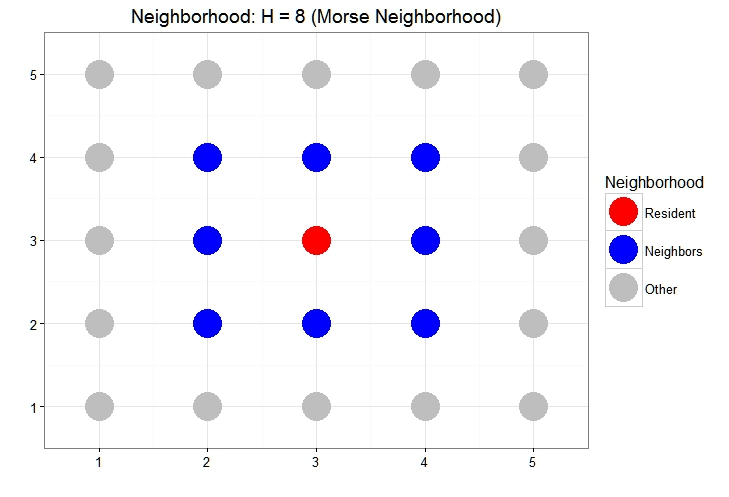
\includegraphics[scale=.33]{figures/H8.jpeg}
\caption{Diagram of Morse Neighborhood}
\label{fig:morse}
\end{figure}

At each step, all the agents simultaneously look at their neighborhood to calculate their ratio of matching race. If that ratio is smaller than the minimum tolerance level, then the agent is \textit{unsatisfied}. All \textit{unsatisfied} agents are simultaneously removed from the board. In Schelling, the agents are placed back into the board randomly, as in Algorithm \ref{alg:euclid}. Luckily, the complexity of the algorithm is $O(n^2)$ at each step. However, at high tolerance levels, the number of steps the algorithm takes grows quickly. For this reason, we run the algorithm until there is at most 10\% \textit{unsatisfied} agents.

 \begin{algorithm}[h!]
  \caption{Schelling Process}\label{alg:euclid}
  \begin{algorithmic}[1]
  	\Function{Schelling}{$agents, grid, tolerance$}\Comment{Agents are defined by their race}
   		\Procedure{Satisfaction}{$agent_i, subgrid, tolerance$}\Comment{The $subgrid$ is a Morse neighborhood of $agent_i$}
        	\State Let $sat = \frac{\mbox{matching agents in $subgrid$ to $agent_i$}}{\mbox{size of subgrid}}$
       		\If {$tolerance < sat $}
       			\State return $TRUE$. \Comment{The agent is $satisfied$.}
                \Else \ return $FALSE$. \Comment{The agent is $unsatisfied$.}
    		\EndIf
        \EndProcedure
    	\While{for any $agent_i$, if Satisfaction is FALSE}
        	\State Remove all $unsatisfied$ agents
            \State Place all $unsatisfied$ agents into randomly assigned empty spots on the grid
        \EndWhile{}
  	\EndFunction{}
  \end{algorithmic}
  \end{algorithm}
  \begin{figure}[h!]
  \caption{Algorithm of Schelling Process}
\end{figure}

It is worth noting that the Schelling algorithm can also be presented as a Markov Chain, although with a complicated transition matrix. At each vertex, each house on the board has some probability $p$ of being race $r$ or vacant ($r=0$). While moving from each state is non-trivial, if we already know which agents are satisfied then the transition matrix is more simple. Hence, we may imagine an initial matrix state $M_{i=0}$. All the odd states remove the previously \textit{unsatisfied} agents and replace them with vacant houses. All the even states return the \textit{unsatisfied} agents to $M$. This may be represented as the following figures from left to right:

\begin{figure}[h!]
\centering

{%
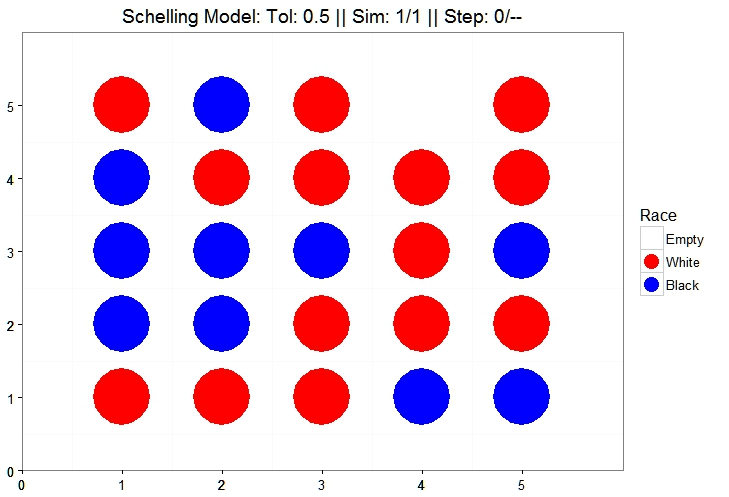
\includegraphics[scale=0.23]{figures/EX0.jpeg}
}
{%
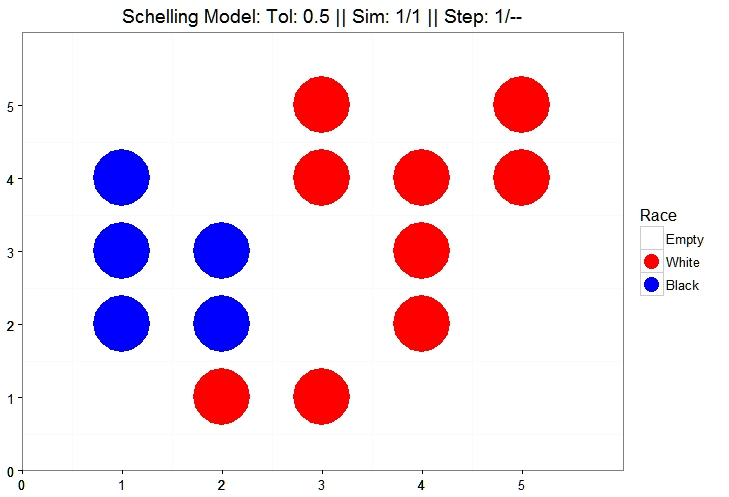
\includegraphics[scale=0.23]{figures/Ex1.jpeg}
}
{%
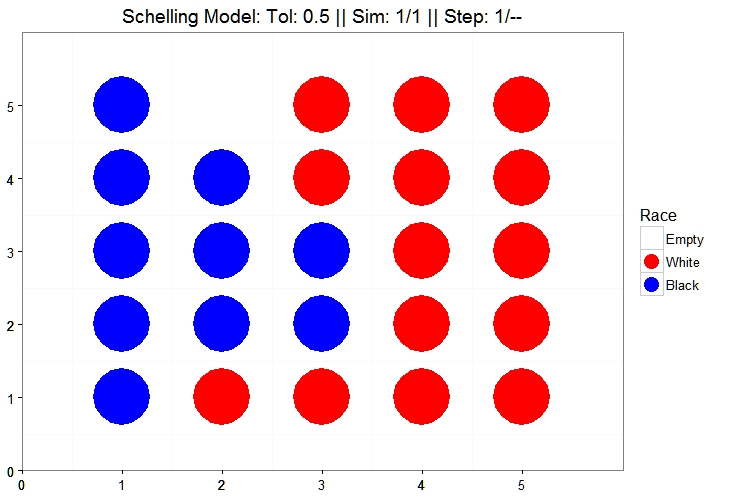
\includegraphics[scale=0.23]{figures/Ex2.jpeg}
}

\caption[Example of Schelling Process]{Example of Schelling: $\tau = 50\%,\ M_{i=0} \rightarrow M_{i=2}$}
\end{figure}

The model in this paper adds a housing gradient as well as a wealth distribution to the original Schelling algorithm.

\subsection{Schelling with a Housing Market}

The housing market is a simple lottery. We take a housing price gradient as given from the data to rank the houses and rank the agents in order of wealth. The agents choose lexicographically with higher wealth agents choosing higher-priced houses. We look at the census tract data for median housing evaluation in Chicago for 2000 and 2010 to model the housing gradient. Spaces can also be empty, allowing the model to have neighborhoods that are more ``urban'' \textit{i.e.} have fewer empty dots, and to somewhat simulate urban decay. All this information is found in the 2000 and 2010 census tract data. Currently, the model does not attempt to simulate differing density levels. They may be done by using the continuous Schelling algorithm, however, this does slow the algorithm.

\begin{figure}[h!]
\centering
\begin{subfigure}{.45\textwidth}
  \centering
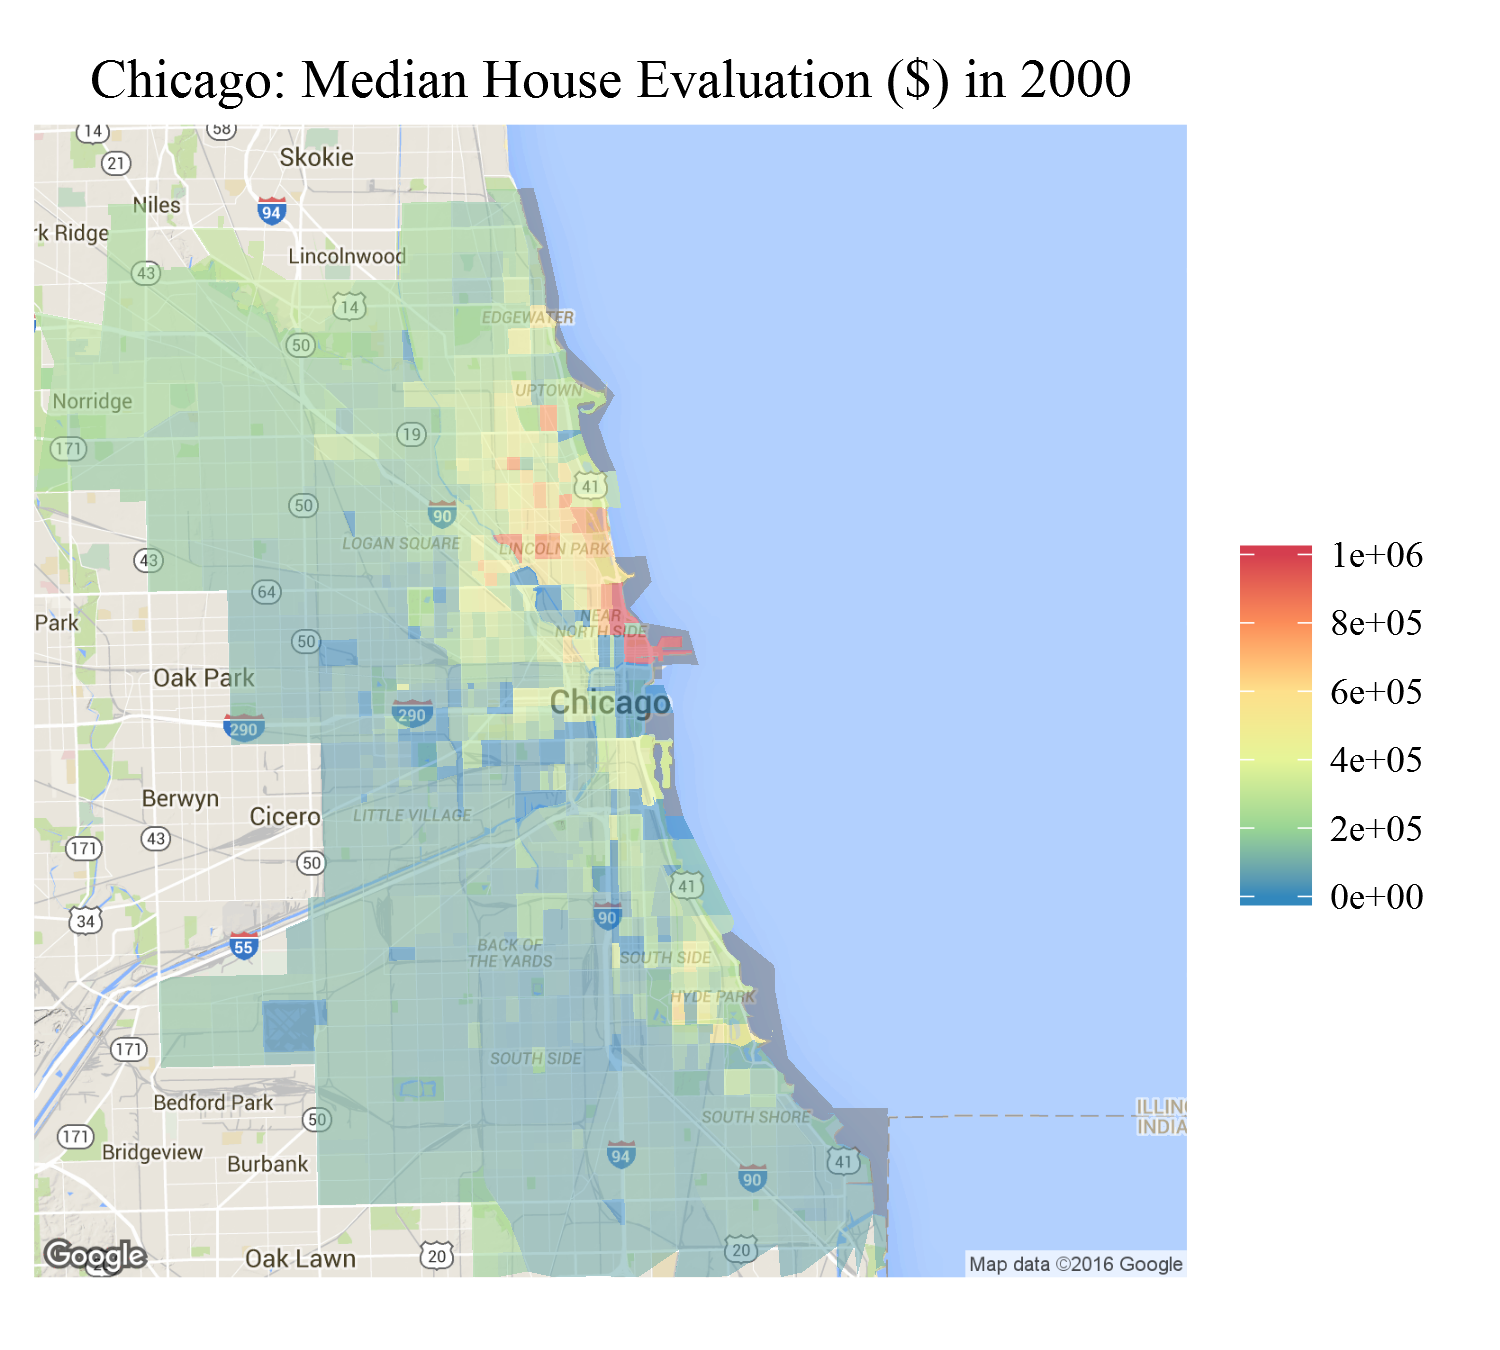
\includegraphics[scale=.15]{figures/c_2000.png}
\end{subfigure}%
\begin{subfigure}{.45\textwidth}
  \centering
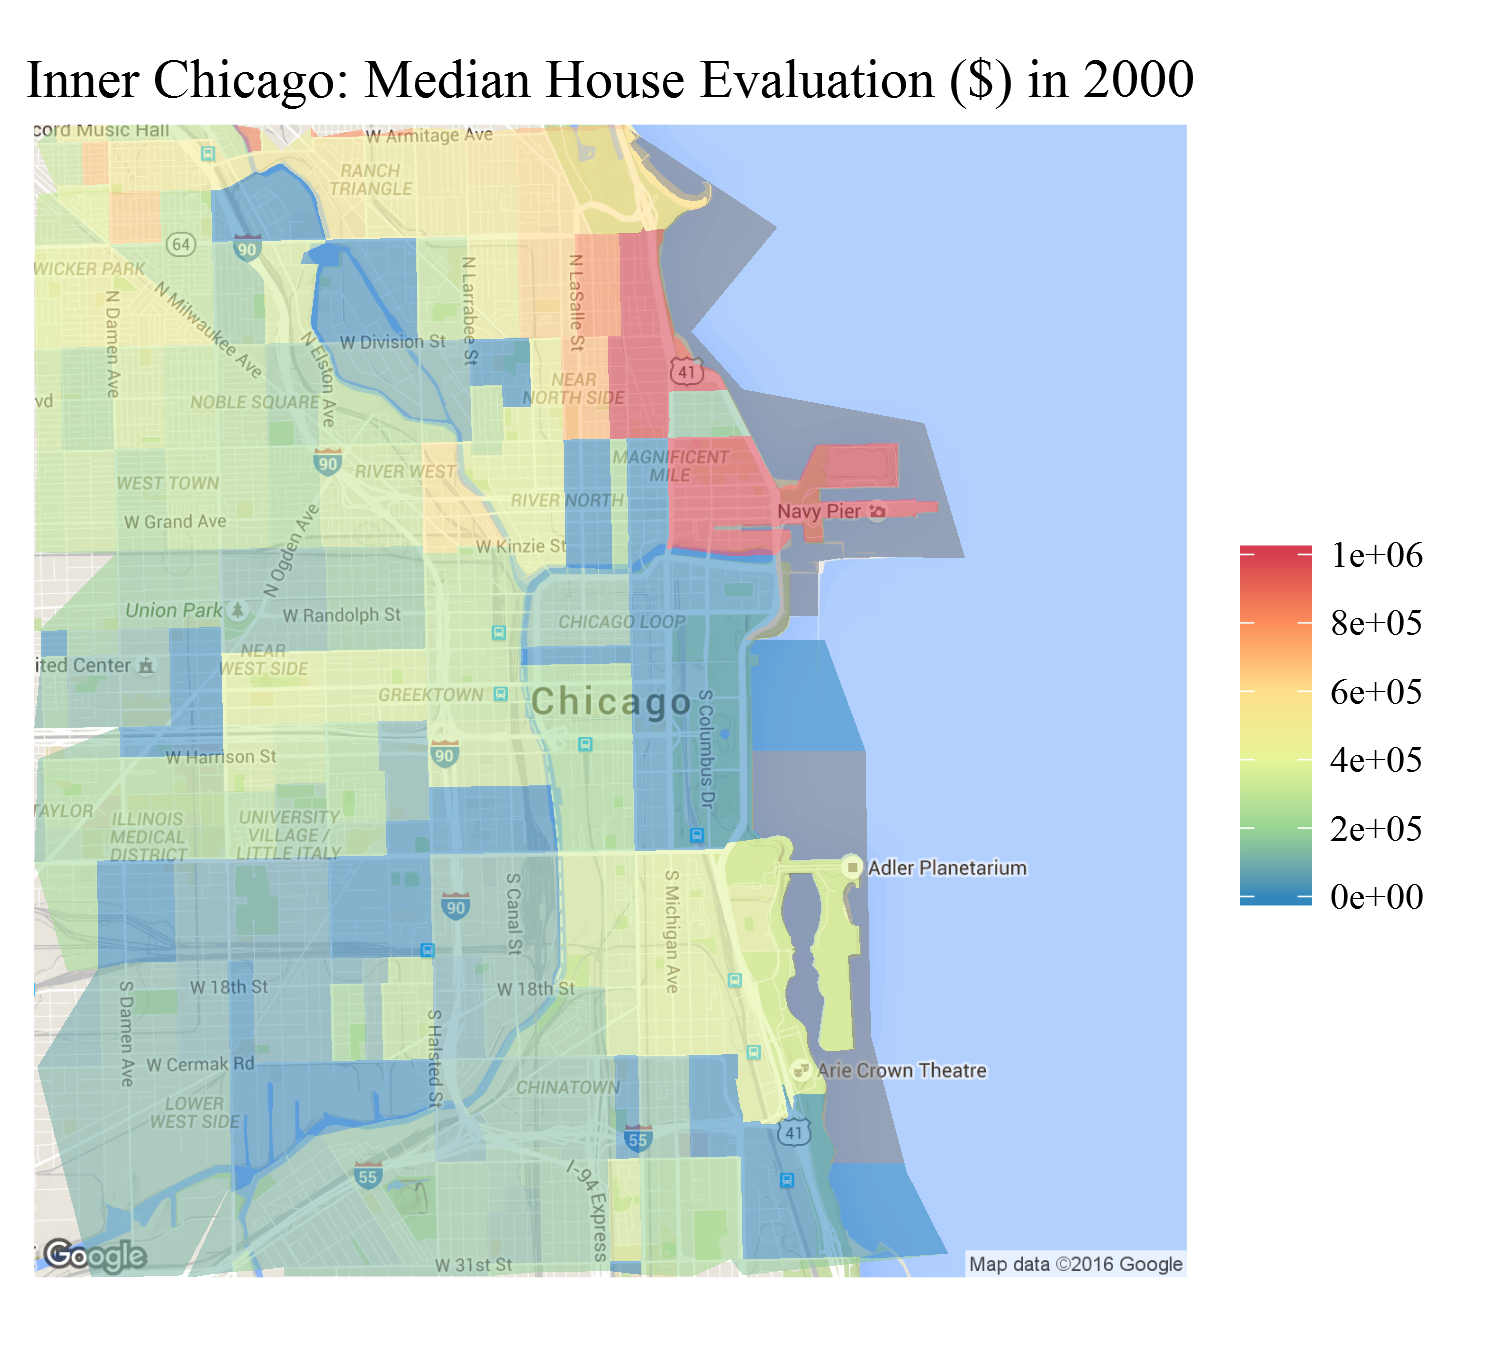
\includegraphics[scale=.15]{figures/c_2000_inner.png}
\end{subfigure}
\label{fig:chicago2000}
\begin{subfigure}{.45\textwidth}
  \centering
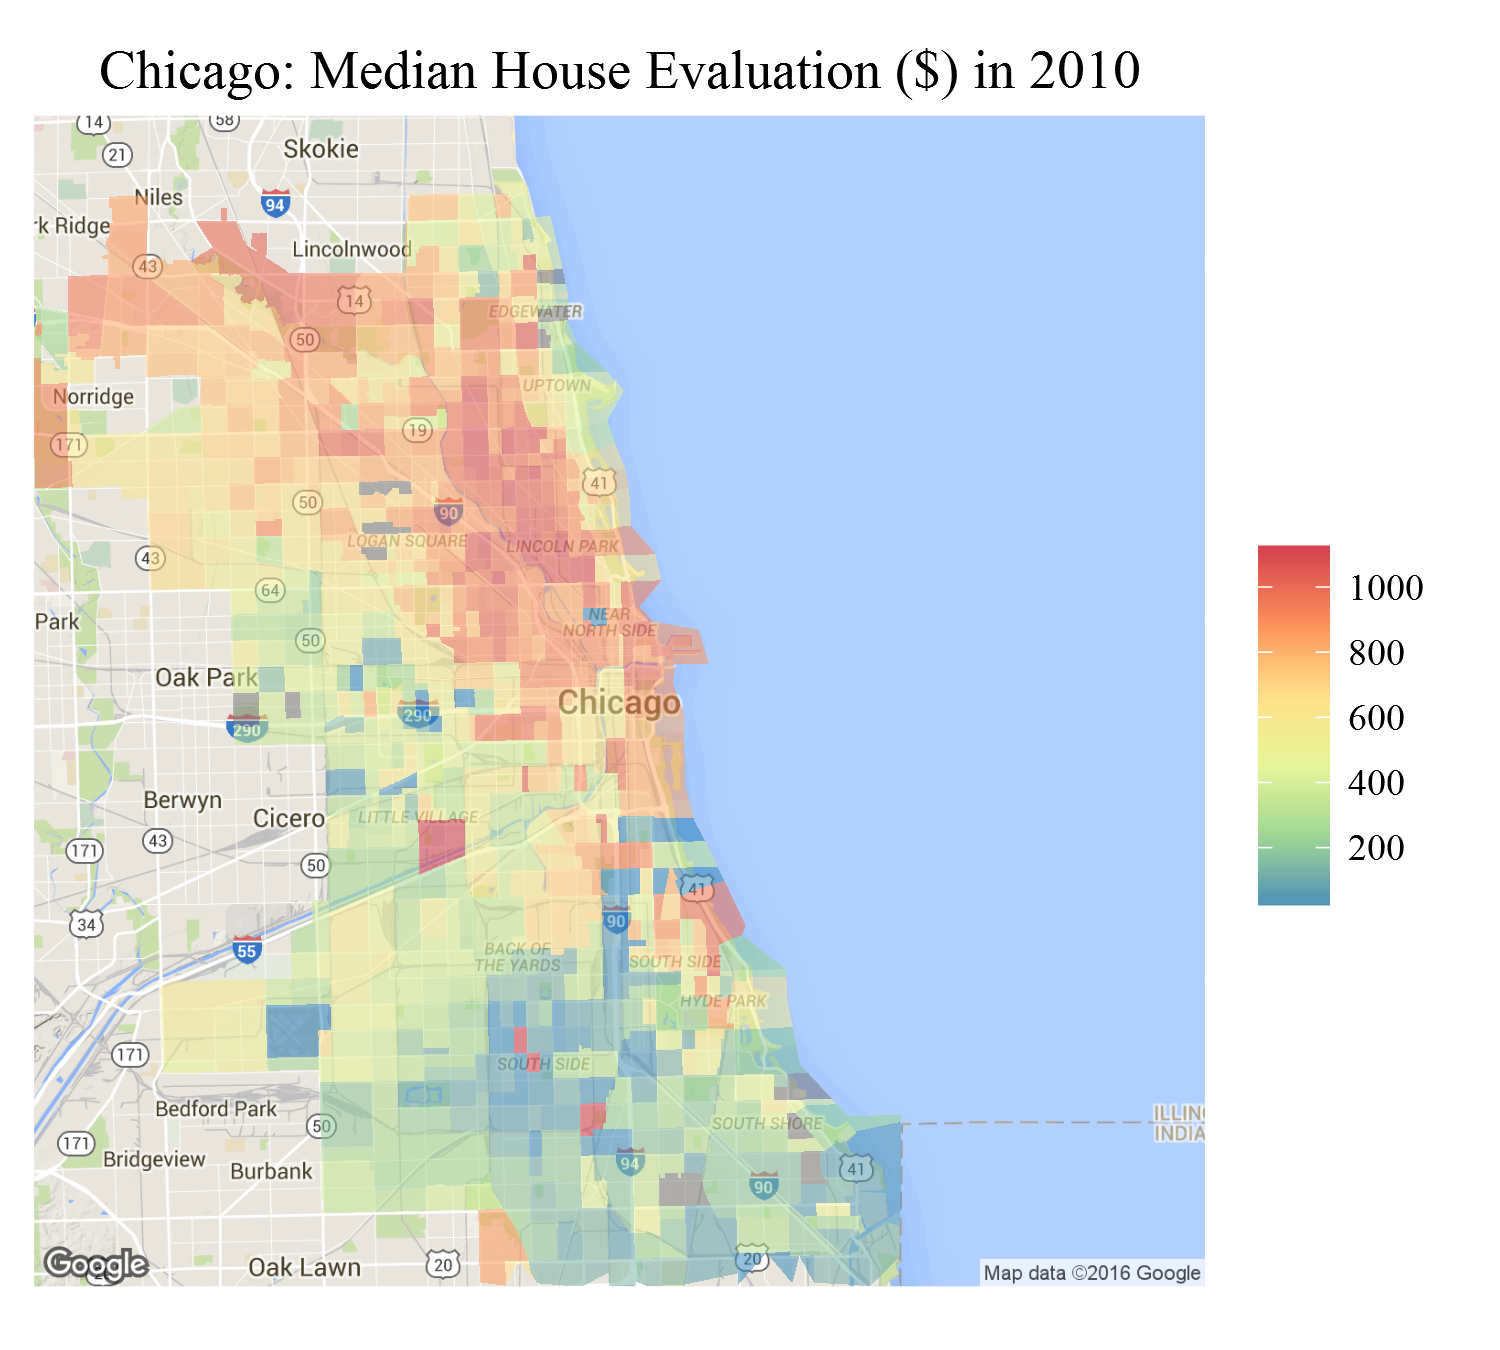
\includegraphics[scale=.15]{figures/c_2010.png}
\end{subfigure}%
\begin{subfigure}{.45\textwidth}
  \centering
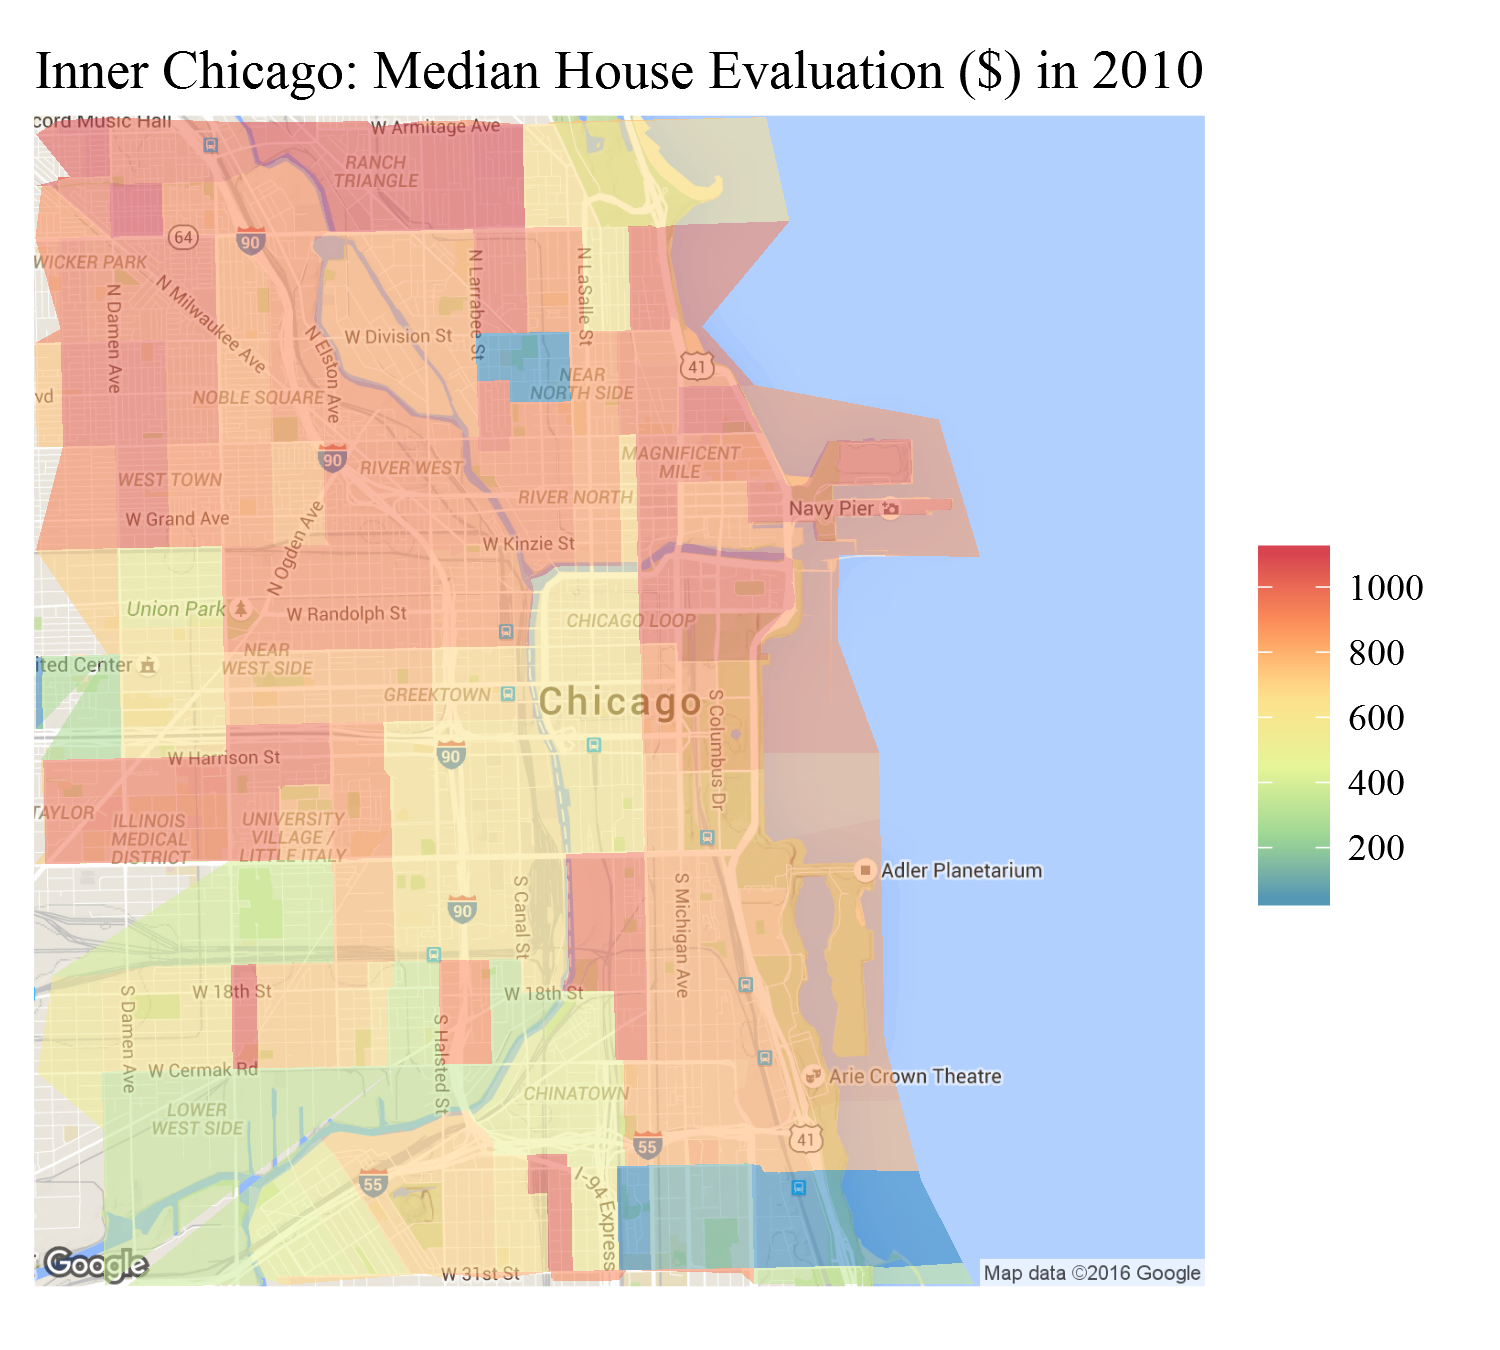
\includegraphics[scale=.15]{figures/c_2010_inner.png}
\end{subfigure}
\caption[Chicago Median Housing Evaluation, 2000-2010]{Chicago: Median Housing Evaluation (\$) in 2000 and 2010}
\label{fig:chicago2000}
\end{figure}

As one may note with Figure \ref{fig:chicago2000} below, the monocentric model of cities in urban economics roughly fits for Chicago \citep{brueckner87}. The center of the city is the most valued and house prices decay outward. However, within the city, there are several instances of high wealth next to low wealth. Urban Economists have a difficult time explaining why there is low wealth accumulation within the city center. Some researchers claim it is due to a combination of larger houses in the suburbs as well as access to better transportation \citep{glaeser08a}. The low wealth individual may only use public transportation while higher wealth individuals own their car(s). Both of these claims may be incorporated into the algorithm in future papers. This may be residual from the 1960s white flight where white people 'retreated' from the more mixed inner city neighborhoods to the mostly white suburbs. The algorithm developed in this paper may be used to analyze the transition, however, the algorithm is missing the structural racism that was present during this time period\citep{cutler97, cutler99}. Similarly, the algorithm is somewhat invariant to initial conditions\citep{zhang11}. It is not clear whether neighborhoods ought to be invariant or whether they are time dependent. Several authors have modeled the housing market with different lags and it is not clear how many lags a housing market may have\citep{glaeser07}. Other tipping algorithms have looked into studying this problem with mixed results\citep{card07}.

\begin{figure}[h!]
\centering
    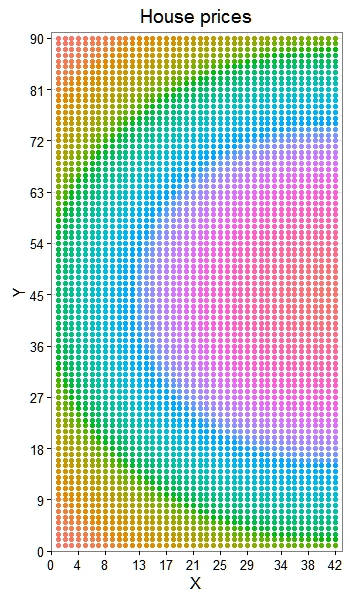
\includegraphics[scale=0.6]{figures/House_Price.jpeg}
    \caption[Simulated Housing Gradient Evaluation]{Simulated Housing Gradient Evaluation. More purple colors mean higher housing values. More red colors mean lower housing values. The decay in evaluation is defined by a euclidean distance}
\end{figure}


In 2010, the highest valued plot of land in Chicago moved northwest from the center. For now, we will assume that there is strict linear decay in the model for both 2000 and 2010. The housing gradient evaluation is simply a Euclidean distance from the center right of the plane. In future papers, one may need to construct a better fitting valuation gradient to better match the city being fitted. This paper does not analyze the robustness of precision of the price gradient. Similarly, upgrading the resolution using a Pointillist map may better capture the underlying distribution. This is especially true for cities which are currently gentrifying or have natural boundaries that create nonlinear (and/or even non-monotonic) price gradients. However, it is also worth noting that the housing market is only interested in ranking. Hence, changing the metric or the $2^{nd}$ derivative of price with respects to space should not change the ranking at all.

This paper modifies the algorithm to incorporate the housing market. Agents still only observe the race of other agents to determine whether they are satisfied. However, now \textit{unsatisfied} agents are sorted back lexicographically into the grid by their wealth. Specifically, agents are sorted by wealth and agents with higher wealth choose higher priced (or valued) houses. This process is described by Algorithm \ref{alg:extendschelling} below. This process allows for better clumping of wealthy agents. However, it allows for clumping of wealth agents in non-central locations. The complexity remains at $O(n^2)$ and there is not much change to the constant term in the complexity.

 \begin{algorithm}[htbp!]
  \caption{Extended Schelling Process}\label{alg:extendschelling}
  \begin{algorithmic}[1]
  	\Function{Extended Schelling}{$agents, grid, tolerance$}\Comment{Race and wealth define the agents.}
   		\Procedure{Satisfaction}{$agent_i, subgrid, tolerance$}\Comment{$subgrid$ is a Morse neighborhood of $agent_i$.}
        	\State Let $sat = \frac{\mbox{matching agents in $subgrid$ to $agent_i$}}{\mbox{size of subgrid}}$
       		\If {$tolerance < sat $}
       			\State return $TRUE$. \Comment{The agent is $satisfied$.}
                \Else \ return $FALSE$. \Comment{The agent is $unsatisfied$.}
    		\EndIf
        \EndProcedure
    	\While{for any $agent_i$, if Satisfaction is FALSE}
        	\State Remove all $unsatisfied$ agents from grid.
            \State Rank all $unsatisfied$ agents by wealth.
            \State Rank all grid spots by the housing price index.
            \State Place all $unsatisfied$ agents in order of wealth to the most valuable real estate on grid.
        \EndWhile{}
  	\EndFunction{}
  \end{algorithmic}
  \end{algorithm}
  \begin{figure}[h!]
\caption{Algorithm of Extended Schelling Process}
\end{figure}

\begin{figure}[h!]
\centering
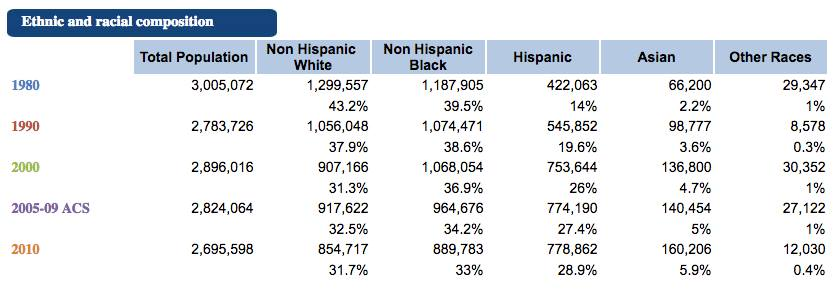
\includegraphics[scale=0.45]{figures/chart4.png}
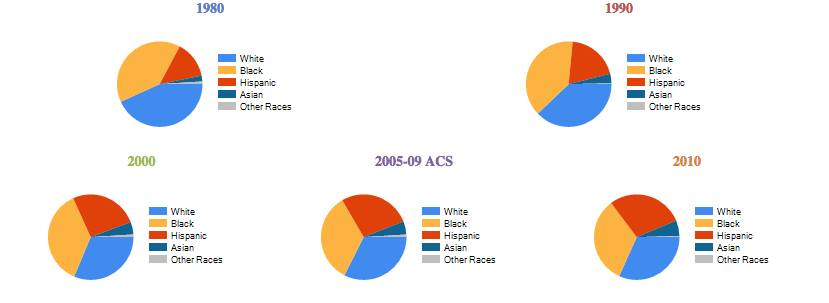
\includegraphics[scale=0.4]{figures/chart3.png}
\caption[Demographics of Chicago]{Demographics of Chicago (Source: US2010)\citep{brown10}}
\label{tab:chicago2}
\end{figure}


The extended Schelling algorithm, by virtue of incorporating both race and wealth, requires a distribution of race and wealth within the population. In fact, the extended algorithm allows for some nuance in the distribution, including individual wealth distribution by race. This allows the extended Schelling algorithm to incorporate the significant wealth differences between races. Figure \ref{tab:chicago2} shows the racial makeup of Chicago in 2000 and 2010. Table \ref{tab:chicago} shows the adjusted racial and wealth make up of Chicago in 2000 and 2010 for the simulation. Races with less than 10\% of the population were dropped as Schelling has difficulty modeling with such low numbers. The wealth distribution represents the fraction of individuals with wealth in the categories described by $w(x)$ in Equation \ref{eq:w}. Note that incomes generally moved up. These incomes, however, are not adjusted for inflation. Census tracts only provide ranges of income, so there is no way to correct for inflation because there is not enough resolution to correctly adjust the category of the edge cases. However, noting that all races saw about 5\% of the population move from income 1 to income 2, it is likely that inflation accounts for much of this change. This effect is different for Whites than for nonwhites, however. Nonwhites saw about 5\% of individuals move from income 2 to income 3, but Whites saw nearly 15\% make that jump.

\begin{table}[h!]
\centering
\caption{Demographics of Chicago}
\label{tab:chicago}
\scalebox{1}{
\begin{tabular}{lllll}
\hline
\multicolumn{5}{l}{Demographics of Chicago Used in Simulations}                                                        \\ \hline \hline
\multicolumn{1}{l|}{Year}     & \multicolumn{2}{l|}{2000}                       & \multicolumn{2}{l}{2010}   \\ \hline
\multicolumn{1}{l|}{Race}     & Population Ratio & \multicolumn{1}{l|}{Wealth Distribution}  & Population Ratio & Wealth Distribution  \\
\multicolumn{1}{l|}{White}    & 60\%           & \multicolumn{1}{l|}{30\%|50\%|20\%} & 56\%            & 25\%|41\%|34\%  \\
\multicolumn{1}{l|}{Black}    & 26\%           & \multicolumn{1}{l|}{53\%|40\%|07\%} & 27\%            & 49\%|40\%|11\%  \\
\multicolumn{1}{l|}{Hispanic} & 14\%           & \multicolumn{1}{l|}{43\%|50\%|07\%} & 17\%            & 37\%|51\%|12\%  \\ \hline \hline
\end{tabular}
}
\end{table}

Other than the significant increase in White wealth, the demographics of Chicago show mostly stable trends from 2000 to 2010. There is a 5\% upwards income drift and a slight decrease in the white population as a share. Asians and other small mass races are excluded from this analysis; the population ratio is the ratio of Chicago's White, Black, and Hispanic population, not the share of its total population. By simulating Chicago with the 2000 and 2010 demographics, one can see whether similar tolerance levels reproduce Chicago's actual segregation statistics on average. If the tolerance level $\tau$ decreases, then this simulation would be evidence of Chicago becoming more racially tolerant. 

\subsection{Estimation}

To estimate the tolerance level in Chicago, this paper simulates the sorting process through the extended Schelling algorithm and then matches several racial segregation indices to Chicago. Widely used by Urban Economists and Sociologists, the Racial Isolation Index and Racial Dissimilarity Index measure different aspects of segregation. The racial isolation index reflects the probability that a minority person lives nears a majority person or with another minority person. The dissimilarity index measures the percentage of a group's population that would have to change residences for each neighborhood to have the same percentage of that group as the metropolitan area overall. Other potential measures of segregation include the Gini coefficient, entropy, and concentration. However, these measures require data with higher resolution than Census tracts. Racial Isolation (``RII'') and Dissimilarity (``RDI'') are calculated as in Equations \ref{eq:rii} and \ref{eq:rdi}, respectively. For the RDI, the ``other race'' is calculated for race $r$ with ``not-$r$'' as the other race \citep{cutler99}.

The simulated city of Chicago is a 90 $\times$ 42 matrix where 92\% of houses are occuppied with a house price gradient evaluation. This matrix was chosen as it has a similar shape and similar amount of vacant house to Chicago. Additionally, neighborhoods do not overlap when we using the Morse neighborhood concept. As previously stated, agents are defined by race and wealth. With 2.896 million people in 2000 and 2.698 million people in 2010, each agent in the model represents $\sim$700 people. Using a Intel(R) Core(TM) i7-5500U CPU @ 2.40GHz, 2401 Mhz, 2 Core(s), 4 Logical Processor(s) in Rstudio Version 0.99.896, the total time for all simulations (both years) was $\sim$ 14 hours. Most of the time was actually taken up by the $\tau = 40\%$ and  $\tau = 50\%$ simulations, which in total took $\sim$ 8.2 hours, over 50\% of the total computation time. This is because more Schelling steps are required at higher tolerance levels and the number of Schelling steps required grows quickly. For this reason, the simulation was stopped at the first step for which less than 10\% \textit{unsatisfied} agents remained. Without that constraint, the process could have continued for an indefinite period of time. Potentially, this constraint biases the segregation indices downwards because some of the final steps, during which further segregation might occur, are not realized. 

\subsection{Results}

This paper runs 100 simulations for each tolerance level with each racial and wealth makeup of Chicago. For each simulation, the racial segregation statistics are calculated and stored. The tables below are summary tables for the racial segregation statistics.

\begin{table}[h!]
\centering
\caption[Racial Isolation, 2000 makeup of Chicago]{Racial Isolation Index for varying Tolerance levels in 2000 makeup of Chicago}
\label{RII.2000}
\scalebox{0.85}{
\begin{tabular}{lllllllllllll}
\hline
\multicolumn{13}{l}{Racial Isolation Index for varying Tolerance levels in 2000 makeup of Chicago} \\ \hline \hline
\multicolumn{1}{l|}{}         & \multicolumn{4}{l|}{$\tau = 0\%$}            & \multicolumn{4}{l|}{$\tau = 10\%$}           & \multicolumn{4}{l}{$\tau = 20\%$} \\ \cline{2-13} 
\multicolumn{1}{l|}{}         & Mean & S.D. & Min & \multicolumn{1}{l|}{Max} & Mean & S.D. & Min & \multicolumn{1}{l|}{Max} & Mean    & S.D.    & Min    & Max   \\ \hline
\multicolumn{1}{l|}{White}    & $0.388$ & $0.018$ & $0.329$ & \multicolumn{1}{l|}{$0.433$} & $0.403$ & $0.017$ & $0.366$ & \multicolumn{1}{l|}{$0.451$} & $0.484$ & $0.024$ & $0.434$ & $0.550$\\
\multicolumn{1}{l|}{Black}    & $0.126$ & $0.014$ & $0.092$ & \multicolumn{1}{l|}{$0.172$} & $0.155$ & $0.016$ & $0.116$ & \multicolumn{1}{l|}{$0.198$} & $0.316$ & $0.029$ & $0.257$ & $0.401$\\
\multicolumn{1}{l|}{Hispanic} & $0.062$ & $0.011$ & $0.035$ & \multicolumn{1}{l|}{$0.094$} & $0.091$ & $0.015$ & $0.053$ & \multicolumn{1}{l|}{$0.129$} & $0.194$ & $0.028$ & $0.145$ & $0.254$\\ \hline
\multicolumn{1}{l|}{}         & \multicolumn{4}{l|}{$\tau = 30\%$}           & \multicolumn{4}{l|}{$\tau = 40\%$}           & \multicolumn{4}{l}{$\tau = 50\%$} \\ \cline{2-13} 
\multicolumn{1}{l|}{}         & Mean & S.D. & Min & \multicolumn{1}{l|}{Max} & Mean & S.D. & Min & \multicolumn{1}{l|}{Max} & Mean    & S.D.    & Min    & Max   \\ \hline
\multicolumn{1}{l|}{White}    & $0.609$ & $0.023$ & $0.554$ & \multicolumn{1}{l|}{$0.661$} & $0.729$ & $0.022$ & $0.681$ & \multicolumn{1}{l|}{$0.787$} & $0.829$ & $0.024$ & $0.773$ & $0.881$ \\
\multicolumn{1}{l|}{Black}    & $0.489$ & $0.029$ & $0.402$ & \multicolumn{1}{l|}{$0.559$} & $0.602$ & $0.033$ & $0.508$ & \multicolumn{1}{l|}{$0.718$} & $0.710$ & $0.036$ & $0.629$ & $0.795$ \\
\multicolumn{1}{l|}{Hispanic} & $0.286$ & $0.036$ & $0.205$ & \multicolumn{1}{l|}{$0.377$} & $0.464$ & $0.038$ & $0.388$ & \multicolumn{1}{l|}{$0.554$} & $0.624$ & $0.046$ & $0.504$ & $0.724$ \\ \hline \hline
\end{tabular}
}
\end{table}

Table \ref{RII.2000} presents the RII for the 2000 make of Chicago. One can see that the mean for the index increases monotonically when the tolerance level increases. This means that as individuals have a higher taste for segregation, cities become more segregated. The bounds of the index are quite small, which allows us to make more precise inferences. There is only slight overlapping between the chosen tolerance levels, and the means monotonically increase with tolerance levels. Interestingly, the RII is both lower and varies more for races that are a small fraction of the population. This is a common critique of this measure, but not of the RDI, which is invariant to population size. However, given the sample size and distribution, as well as the tight bounds, these statistics can be accepted with high confidence. We find similar results for for table \ref{RII.2010}.

\begin{table}[h!]
\centering
\caption[Racial Dissimilarity, 2000 makeup of Chicago]{Racial Dissimilarity Index for varying Tolerance levels in 2000 makeup of Chicago}
\label{RDI.2000}
\scalebox{0.85}{
\begin{tabular}{lllllllllllll}
\hline
\multicolumn{13}{l}{Racial Dissimilarity Index for varying Tolerance levels in 2000 makeup of Chicago} \\ \hline \hline
\multicolumn{1}{l|}{}         & \multicolumn{4}{l|}{$\tau = 0\%$}            & \multicolumn{4}{l|}{$\tau = 10\%$}           & \multicolumn{4}{l}{$\tau = 20\%$} \\ \cline{2-13} 
\multicolumn{1}{l|}{}         & Mean & S.D. & Min & \multicolumn{1}{l|}{Max} & Mean & S.D. & Min & \multicolumn{1}{l|}{Max} & Mean    & S.D.    & Min    & Max   \\ \hline
\multicolumn{1}{l|}{White}    & $0.240$ & $0.085$ & $0.156$ & \multicolumn{1}{l|}{$0.371$} & $0.240$ & $0.084$ & $0.158$ & \multicolumn{1}{l|}{$0.397$} & $0.288$ & $0.103$ & $0.197$ & $0.469$ \\
\multicolumn{1}{l|}{Black}    & $0.168$ & $0.044$ & $0.082$ & \multicolumn{1}{l|}{$0.241$} & $0.158$ & $0.042$ & $0.073$ & \multicolumn{1}{l|}{$0.229$} & $0.260$ & $0.071$ & $0.126$ & $0.379$ \\
\multicolumn{1}{l|}{Hispanic} & $0.095$ & $0.025$ & $0.043$ & \multicolumn{1}{l|}{$0.148$} & $0.134$ & $0.033$ & $0.055$ & \multicolumn{1}{l|}{$0.196$} & $0.250$ & $0.042$ & $0.126$ & $0.333$ \\ \hline
\multicolumn{1}{l|}{}         & \multicolumn{4}{l|}{$\tau = 30\%$}           & \multicolumn{4}{l|}{$\tau = 40\%$}           & \multicolumn{4}{l}{$\tau = 50\%$} \\ \cline{2-13} 
\multicolumn{1}{l|}{}         & Mean & S.D. & Min & \multicolumn{1}{l|}{Max} & Mean & S.D. & Min & \multicolumn{1}{l|}{Max} & Mean    & S.D.    & Min    & Max   \\ \hline
\multicolumn{1}{l|}{White}    & $0.387$ & $0.136$ & $0.249$ & \multicolumn{1}{l|}{$0.599$} & $0.592$ & $0.188$ & $0.353$ & \multicolumn{1}{l|}{$0.794$ } & $0.576$ & $0.194$ & $0.352$ & $0.796$ \\
\multicolumn{1}{l|}{Black}    & $0.385$ & $0.107$ & $0.201$ & \multicolumn{1}{l|}{$0.509$} & $0.531$ & $0.167$ & $0.287$ & \multicolumn{1}{l|}{$0.727$}  & $0.515$ & $0.170$ & $0.278$ & $0.727$ \\
\multicolumn{1}{l|}{Hispanic} & $0.327$ & $0.063$ & $0.143$ & \multicolumn{1}{l|}{$0.432$} & $0.556$ & $0.136$ & $0.256$ & \multicolumn{1}{l|}{$0.723$}  & $0.527$ & $0.104$ & $0.240$ & $0.649$ \\ \hline \hline
\end{tabular}
}
\end{table}

In contrast to Table \ref{RII.2000}, Table \ref{RDI.2000} has a much larger standard deviation. The indexes at several tolerance levels overlap each other. However, this reflects the randomness inherent in a Schelling process. As the figures in the Appendix show, there is sometimes large variance in the number of matching agents within a neighborhood. This is especially true for smaller demographics, such as Hispanics or Wealthy agents. Although the means monotonically increase, there is a big jump between 30\% and 40\%. The standard deviations do not increase much with the means, which increases the confidence in the estimated increase in segregation.

\begin{table}[h!]
\centering
\caption[Racial Isolation, 2010 makeup of Chicago]{Racial Isolation Index for varying Tolerance levels in 2010 makeup of Chicago}
\label{RII.2010}
\scalebox{0.85}{
\begin{tabular}{lllllllllllll}
\hline
\multicolumn{13}{l}{Racial Isolation Index for varying Tolerance levels in 2010 makeup of Chicago} \\ \hline \hline
\multicolumn{1}{l|}{}         & \multicolumn{4}{l|}{$\tau = 0\%$}            & \multicolumn{4}{l|}{$\tau = 10\%$}           & \multicolumn{4}{l}{$\tau = 20\%$} \\ \cline{2-13} 
\multicolumn{1}{l|}{}         & Mean & S.D. & Min & \multicolumn{1}{l|}{Max} & Mean & S.D. & Min & \multicolumn{1}{l|}{Max} & Mean    & S.D.    & Min   & Max   \\ \hline
\multicolumn{1}{l|}{White}    & $0.350$ & $0.020$ & $0.310$ & \multicolumn{1}{l|}{$0.401$} & $0.365$ & $0.020$ & $0.300$ & \multicolumn{1}{l|}{$0.402$} & $0.459$ & $0.022$ & $0.394$ & $0.502$ \\
\multicolumn{1}{l|}{Black}    & $0.126$ & $0.014$ & $0.092$ & \multicolumn{1}{l|}{$0.167$} & $0.165$ & $0.018$ & $0.124$ & \multicolumn{1}{l|}{$0.212$} & $0.316$ & $0.027$ & $0.254$ & $0.386$ \\
\multicolumn{1}{l|}{Hispanic} & $0.075$ & $0.012$ & $0.048$ & \multicolumn{1}{l|}{$0.106$} & $0.111$ & $0.017$ & $0.070$ & \multicolumn{1}{l|}{$0.165$} & $0.226$ & $0.026$ & $0.148$ & $0.274$ \\ \hline
\multicolumn{1}{l|}{}         & \multicolumn{4}{l|}{$\tau = 30\%$}           & \multicolumn{4}{l|}{$\tau = 40\%$}           & \multicolumn{4}{l}{$\tau = 50\%$} \\ \cline{2-13} 
\multicolumn{1}{l|}{}         & Mean & S.D. & Min & \multicolumn{1}{l|}{Max} & Mean & S.D. & Min & \multicolumn{1}{l|}{Max} & Mean    & S.D.    & Min    & Max   \\ \hline
\multicolumn{1}{l|}{White}    & $0.599$ & $0.024$ & $0.518$ & \multicolumn{1}{l|}{$0.651$} & $0.729$ & $0.023$ & $0.662$ & \multicolumn{1}{l|}{$0.782$} & $0.830$ & $0.022$ & $0.782$ & $0.895$ \\
\multicolumn{1}{l|}{Black}    & $0.482$ & $0.029$ & $0.403$ & \multicolumn{1}{l|}{$0.556$} & $0.599$ & $0.033$ & $0.531$ & \multicolumn{1}{l|}{$0.680$} & $0.715$ & $0.035$ & $0.632$ & $0.811$ \\
\multicolumn{1}{l|}{Hispanic} & $0.346$ & $0.036$ & $0.263$ & \multicolumn{1}{l|}{$0.428$} & $0.474$ & $0.042$ & $0.365$ & \multicolumn{1}{l|}{$0.584$} & $0.612$ & $0.049$ & $0.471$ & $0.714$ \\ \hline \hline
\end{tabular}
}
\end{table}
\begin{table}[h!]
\centering
\caption[Racial Dissimilarity, 2010 makeup of Chicago]{Racial Dissimilarity Index for varying Tolerance levels in 2010 makeup of Chicago}
\label{RDI.2010}
\scalebox{0.85}{
\begin{tabular}{lllllllllllll}
\hline
\multicolumn{13}{l}{Racial Isolation Index for varying Tolerance levels in 2010 makeup of Chicago} \\ \hline \hline
\multicolumn{1}{l|}{}         & \multicolumn{4}{l|}{$\tau = 0\%$}            & \multicolumn{4}{l|}{$\tau = 10\%$}           & \multicolumn{4}{l}{$\tau = 20\%$} \\ \cline{2-13} 
\multicolumn{1}{l|}{}         & Mean & S.D. & Min & \multicolumn{1}{l|}{Max} & Mean & S.D. & Min & \multicolumn{1}{l|}{Max} & Mean    & S.D.    & Min    & Max   \\ \hline
\multicolumn{1}{l|}{White}    & $0.232$ & $0.079$ & $0.141$ & \multicolumn{1}{l|}{$0.349$} & $0.227$ & $0.080$ & $0.142$ & \multicolumn{1}{l|}{$0.356$} & $0.319$ & $0.104$ & $0.184$ & $0.455$ \\
\multicolumn{1}{l|}{Black}    & $0.151$ & $0.040$ & $0.073$ & \multicolumn{1}{l|}{$0.219$} & $0.151$ & $0.042$ & $0.071$ & \multicolumn{1}{l|}{$0.215$} & $0.248$ & $0.074$ & $0.131$ & $0.358$ \\
\multicolumn{1}{l|}{Hispanic} & $0.099$ & $0.027$ & $0.044$ & \multicolumn{1}{l|}{$0.154$} & $0.142$ & $0.034$ & $0.055$ & \multicolumn{1}{l|}{$0.221$} & $0.254$ & $0.064$ & $0.101$ & $0.337$ \\ \hline
\multicolumn{1}{l|}{}         & \multicolumn{4}{l|}{$\tau = 30\%$}           & \multicolumn{4}{l|}{$\tau = 40\%$}           & \multicolumn{4}{l}{$\tau = 50\%$} \\ \cline{2-13} 
\multicolumn{1}{l|}{}         & Mean & S.D. & Min & \multicolumn{1}{l|}{Max} & Mean & S.D. & Min & \multicolumn{1}{l|}{Max} & Mean    & S.D.    & Min    & Max   \\ \hline
\multicolumn{1}{l|}{White}    & $0.413$ & $0.139$ & $0.237$ & \multicolumn{1}{l|}{$0.599$} & $0.521$ & $0.164$ & $0.312$ & \multicolumn{1}{l|}{$0.711$} & $0.614$ & $0.183$ & $0.353$ & $0.808$ \\
\multicolumn{1}{l|}{Black}    & $0.365$ & $0.108$ & $0.199$ & \multicolumn{1}{l|}{$0.519$} & $0.460$ & $0.135$ & $0.238$ & \multicolumn{1}{l|}{$0.652$} & $0.499$ & $0.172$ & $0.282$ & $0.748$ \\
\multicolumn{1}{l|}{Hispanic} & $0.370$ & $0.075$ & $0.163$ & \multicolumn{1}{l|}{$0.474$} & $0.443$ & $0.113$ & $0.218$ & \multicolumn{1}{l|}{$0.603$} & $0.562$ & $0.124$ & $0.252$ & $0.711$ \\ \hline \hline
\end{tabular}
}
\end{table}

Racial Dissimilarity and Racial Isolation in the following tables both similarly match Chicago's actual 2000 and 2010 values. However, the RII values increase more slowly in tolerance than the RDI values, and the standard deviation of RII is larger. This reflects the differing interpretations of RDI versus RII. RDI is a citywide estimate of the segregation of one race from all other mutually exclusive racial groups, while the RII is a citywide estimate of the segregation of one racial group generally within neighborhoods. The RDI is roughly a measure of how strongly two races clump themselves into largely segregated neighborhoods; this tends to happen quickly, and numerically it is easier for a neighborhood to be largely of one race. The RII, however, is more sensitive to the distribution of one race within a neighborhood, which is more likely to vary because it is more subject to initial conditions. This reflects a peculiarity of the Schelling process; unlike a regular Schelling process, there is not random placement in the city but rather some wealth concentration. Hence, although the wealth inequality drives broader trends in inequality, therefore universally pushing up the RDI, there is still significant random variation within some neighborhoods because, for example, poor Blacks cannot escape into rich White neighborhoods, even if both groups would tolerate that move.

\begin{figure}[!h]
\centering
\begin{subfigure}[b]{.5\textwidth}
  \centering
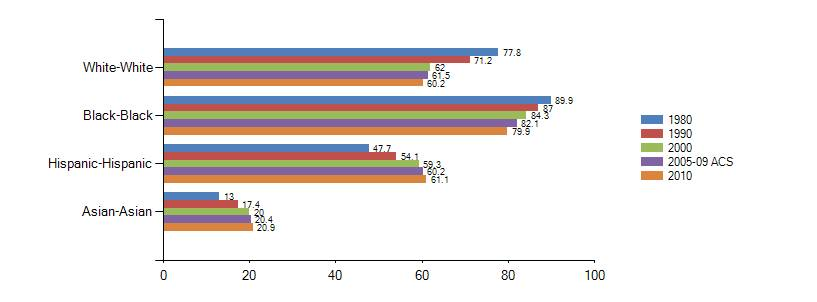
\includegraphics[scale=.35]{figures/chart1.png}
\caption{Racial Dissimilarity Index}
\end{subfigure}%
\begin{subfigure}[b]{.5\textwidth}
  \centering
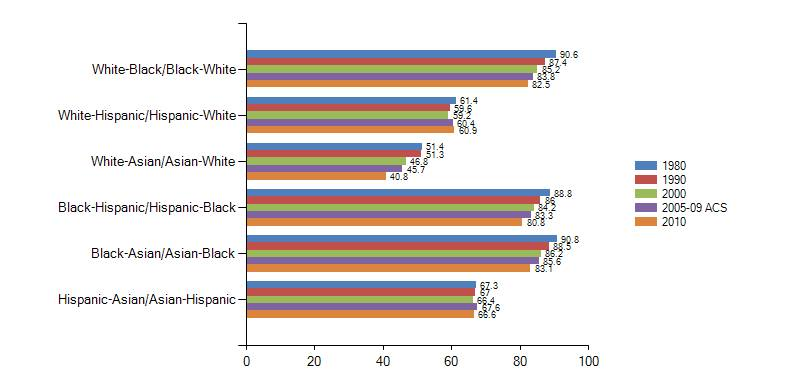
\includegraphics[scale=.35]{figures/chart2.png}
\caption{Racial Isolation Index}
\end{subfigure}
\caption{Actual Segregation Indices for Chicago}
\end{figure}

For both 2000 and 2010 demographics, a 50\% tolerance level is the minimum tolerance level sufficient to reproduce Chicago's segregation statistics on average. Because a 50\% tolerance level is the minimum tolerance level for both parameterizations, we can conclude that if housing choices are made with a Schelling process, Chicago has not become more tolerant in the past decade. Interestingly, 50\% is the amount of housing discrimination the General Social Survey finds that Whites are willing to tolerate, suggesting that there is no ``housing Bradley effect.''\footnote{The Bradley Effect is named for the 1982 California gubernatorial election, in which there was significant response bias to public polling. Bradley, the longtime Los Angeles mayor, lost the election despite leading in the polls. Several have speculated that respondents, despite opposing Bradley, did not want to appear racist in front of pollsters by opposing an ``historic'' election. Therefore, the Bradley Effect has particular racial significance in the context of American politics and public policy beyond polling response bias.} This means that even if Whites are honest about their racial preferences, these relatively benign preferences can result in highly segregated cities, even if the initial conditions are random. In real life, of course, the initial conditions are not randomly distributed; in fact, Chicago is already a highly segregated city, so it is possible that these simulations underestimate how racially tolerant Whites are because the initial conditions are not random. However, Zhang does provide some evidence of invariance to initial conditions in simulation convergence; his proof, however, is not mathematical. In short, more testing and analysis are required.

\subsection{Conclusion}

An extended Schelling process appears to be a somewhat compelling explanation for the underlying dynamics of the Chicago housing market given its ability to reproduce Chicago's level of segregation with the stated preferences of respondents to the General Social Survey. Furthermore, it is surprisingly robust to initial conditions. However, this simulation has room for more complexity motivated by realism.

The current extended Schelling algorithm only has a lower bound level of tolerance. However, it is plausible that there is also an upper bound level of tolerance, as well --- in Beckerian terms, ``taste for diversity.'' Furthermore, tolerance levels are constant across races. In practice, there is significant heterogeneity of racial tolerance for housing segregation, and indeed Blacks seem to have a preference for diversity (or, at least, Whites). Future simulations could easily be built to incorporate these types of heterogeneous preferences. In a similar vein, some cities, like Los Angeles, are not well described by a monocentric price topology. Future simulations could be parameterized to find implied tolerance levels for such cities as well. Although RDI and RII are the most common measures of segregation, future papers could benefit from using more obscure but specialized segregation measures. For example, the Racial Exposure Index could be used to measure racial similarity within neighborhoods.

Similarly, looking at other US cities such as Detroit, Houston, and New York City may better illustrate the underlying racial tensions within cities. Chicago is well-known for its corruption and institutional racism in the 20th century, which potentially enforce segregation more strongly than the heavily migrant cities found in Texas, like Houston. In the same vein, Hispanic and Asian immigrants may radically changed the interaction between races. For example, both Asians and Hispanics tend to either segregate heavily when of low wealth, or integrate heavily when of high wealth. This may be more indicative of the \textit{port of entry} theory of segregation after the \textit{structural racism} began to erode with the removal of the Chinese Exclusion Act in 1943 and recent mass Hispanic immigration.

Most importantly, future simulations can build out a more complex model for agent optimization. Currently, an individual faces no trade-off for investing all of one's income, which is endowed each period with 100\% depreciation, into housing. In reality, individuals have at least partially storable income and face tradeoffs between housing and other forms of consumption, as well as other investment opportunities which affect future income flows. Consumption and investment opportunities are affected by one's housing location, but this type of dependency may not add any clarity worth the loss of tractability. R\'emi Lemoy and Charles Raux et Pablo Jensen present a model that could be used for such future simulations\citep{lemoy10}.  

As this paper shows, however, even honest, benign racial preferences can result in severe segregation exacerbated by wealth inequality. Furthermore, this can occur in the absence of any external pressure from racially motivated policy, past or present. There seems to need to be a preference for diversity if neighborhoods are to desegregate. From a public policy perspective, an ``affirmative action'' policy for neighborhoods is infeasible, but a cultural preference for diversity might not be. Furthermore, governments could institute incentive programs, if not directly for diversity, for factors that correlate with diversity, such as funding for cultural programs but not for close substitutes. This paper confirms Schellings' intuition that the problem of segregation is more difficult than originally conceived. To desegregate, it is not enough solely to \textit{tolerate} other races.


%Note:BibTeX also works

\bibliographystyle{chicago}
\bibliography{references}

\end{document}


